%-*-latex-*-
\sectionthree{Rotations; Self-Balancing AVL BST}
\begin{python0}
from solutions import *; clear()
\end{python0}

\subsection{Left and right rotations}

As I said in previous sections, we want to use search trees to store data
and we want to search for a particular data very quickly.
The number of iterations that must be carried out is at
worse the height of the tree.
So we want the height to be as small as possible.
Which is the same as saying, for the case of a binary search tree,
the height of the left subtree
is roughly the same as the height of the right subtree.

The sense of being height balanced is a definition not just at the root
of the BST, but at every node.
Why?
Because if the tree is not height balanced, then there are two leaves
that will meet at a common ancentor $c$ and the lengths of their
path are significantly different.
The way to \lq\lq repair'' the the tree is to repair the subtree with
root $c$ first.
The operation is more or less to more some nodes from the taller
subtree of $c$ to the shorter subtree.
This is achieved through two operators:
the left rotation and right rotation about a node.

You can define left and right rotations about any node.
So first I'll describe the left and right rotations and then talk about
AVL trees, i.e., height balanced BST.

The following describes the left rotation operation about 
$\alpha$:
\begin{center}
\begin{tikzpicture}

\fill[blue!10] (0.0, 0.0) circle (0.35);
\node [line width=0.03cm,black,minimum size=0.6699999999999999cm,draw,circle] at (0.0,0.0)(1){};\draw (0.0, 0.0) node[color=black] {\texttt{1}};
\fill[blue!10] (-1.9, -1.0) circle (0.35);
\node [line width=0.03cm,black,minimum size=0.6699999999999999cm,draw,circle] at (-1.9,-1.0)(0){};\draw (-1.9, -1.0) node[color=black] {\texttt{0}};
\fill[blue!10] (1.9, -1.0) circle (0.35);
\node [line width=0.03cm,black,minimum size=0.6699999999999999cm,draw,circle] at (1.9,-1.0)(9){};\draw (1.9, -1.0) node[color=black] {\texttt{9}};
\fill[blue!10] (-2.85, -2.0) circle (0.35);
\node [line width=0.03cm,black,minimum size=0.6699999999999999cm,draw,circle] at (-2.85,-2.0)(8){};\draw (-2.85, -2.0) node[color=black] {\texttt{8}};
\fill[blue!10] (-0.95, -2.0) circle (0.35);
\node [line width=0.03cm,black,minimum size=0.6699999999999999cm,draw,circle] at (-0.95,-2.0)(3){};\draw (-0.95, -2.0) node[color=black] {\texttt{3}};
\fill[blue!10] (0.95, -2.0) circle (0.35);
\node [line width=0.03cm,black,minimum size=0.6699999999999999cm,draw,circle] at (0.95,-2.0)(2){};\draw (0.95, -2.0) node[color=black] {\texttt{2}};
\fill[blue!10] (2.85, -2.0) circle (0.35);
\node [line width=0.03cm,black,minimum size=0.6699999999999999cm,draw,circle] at (2.85,-2.0)(4){};\draw (2.85, -2.0) node[color=black] {\texttt{4}};
\fill[blue!10] (-3.33, -3.0) circle (0.35);
\node [line width=0.03cm,black,minimum size=0.6699999999999999cm,draw,circle] at (-3.33,-3.0)(7){};\draw (-3.33, -3.0) node[color=black] {\texttt{7}};
\fill[blue!10] (-2.38, -3.0) circle (0.35);
\node [line width=0.03cm,black,minimum size=0.6699999999999999cm,draw,circle] at (-2.38,-3.0)(6){};\draw (-2.38, -3.0) node[color=black] {\texttt{6}};\draw[line width=0.03cm,black] (1) to  (0);
\draw[line width=0.03cm,black] (1) to  (9);
\draw[line width=0.03cm,black] (0) to  (8);
\draw[line width=0.03cm,black] (0) to  (3);
\draw[line width=0.03cm,black] (9) to  (2);
\draw[line width=0.03cm,black] (9) to  (4);
\draw[line width=0.03cm,black] (8) to  (7);
\draw[line width=0.03cm,black] (8) to  (6);
\node [ellipse, draw=red, fit=(3), line width=0.1cm, inner sep=0.0cm] {};\node [ellipse, draw=red, fit=(2), line width=0.1cm, inner sep=0.0cm] {};\node [ellipse, draw=red, fit=(4), line width=0.1cm, inner sep=0.0cm] {};\node [ellipse, draw=red, fit=(7), line width=0.1cm, inner sep=0.0cm] {};\node [ellipse, draw=red, fit=(6), line width=0.1cm, inner sep=0.0cm] {};
\end{tikzpicture}

\end{center}


\begin{center}
\begin{tikzpicture}

\fill[blue!10] (0.0, 0.0) circle (0.35);
\node [line width=0.03cm,black,minimum size=0.6699999999999999cm,draw,circle] at (0.0,0.0)(1){};\draw (0.0, 0.0) node[color=black] {\texttt{1}};
\fill[blue!10] (-1.9, -1.0) circle (0.35);
\node [line width=0.03cm,black,minimum size=0.6699999999999999cm,draw,circle] at (-1.9,-1.0)(0){};\draw (-1.9, -1.0) node[color=black] {\texttt{0}};
\fill[blue!10] (1.9, -1.0) circle (0.35);
\node [line width=0.03cm,black,minimum size=0.6699999999999999cm,draw,circle] at (1.9,-1.0)(9){};\draw (1.9, -1.0) node[color=black] {\texttt{9}};
\fill[blue!10] (-2.85, -2.0) circle (0.35);
\node [line width=0.03cm,black,minimum size=0.6699999999999999cm,draw,circle] at (-2.85,-2.0)(8){};\draw (-2.85, -2.0) node[color=black] {\texttt{8}};
\fill[blue!10] (-0.95, -2.0) circle (0.35);
\node [line width=0.03cm,black,minimum size=0.6699999999999999cm,draw,circle] at (-0.95,-2.0)(3){};\draw (-0.95, -2.0) node[color=black] {\texttt{3}};
\fill[blue!10] (0.95, -2.0) circle (0.35);
\node [line width=0.03cm,black,minimum size=0.6699999999999999cm,draw,circle] at (0.95,-2.0)(2){};\draw (0.95, -2.0) node[color=black] {\texttt{2}};
\fill[blue!10] (2.85, -2.0) circle (0.35);
\node [line width=0.03cm,black,minimum size=0.6699999999999999cm,draw,circle] at (2.85,-2.0)(4){};\draw (2.85, -2.0) node[color=black] {\texttt{4}};
\fill[blue!10] (-3.33, -3.0) circle (0.35);
\node [line width=0.03cm,black,minimum size=0.6699999999999999cm,draw,circle] at (-3.33,-3.0)(7){};\draw (-3.33, -3.0) node[color=black] {\texttt{7}};
\fill[blue!10] (-2.38, -3.0) circle (0.35);
\node [line width=0.03cm,black,minimum size=0.6699999999999999cm,draw,circle] at (-2.38,-3.0)(6){};\draw (-2.38, -3.0) node[color=black] {\texttt{6}};\draw[line width=0.03cm,black] (1) to  (0);
\draw[line width=0.03cm,black] (1) to  (9);
\draw[line width=0.03cm,black] (0) to  (8);
\draw[line width=0.03cm,black] (0) to  (3);
\draw[line width=0.03cm,black] (9) to  (2);
\draw[line width=0.03cm,black] (9) to  (4);
\draw[line width=0.03cm,black] (8) to  (7);
\draw[line width=0.03cm,black] (8) to  (6);
\node [ellipse, draw=red, fit=(3), line width=0.1cm, inner sep=0.0cm] {};\node [ellipse, draw=red, fit=(2), line width=0.1cm, inner sep=0.0cm] {};\node [ellipse, draw=red, fit=(4), line width=0.1cm, inner sep=0.0cm] {};\node [ellipse, draw=red, fit=(8) (7) (6), line width=0.1cm, inner sep=0.0cm] {};
\end{tikzpicture}

\end{center}


\begin{center}
\begin{tikzpicture}

\fill[blue!10] (0.0, 0.0) circle (0.35);
\node [line width=0.03cm,black,minimum size=0.6699999999999999cm,draw,circle] at (0.0,0.0)(1){};\draw (0.0, 0.0) node[color=black] {\texttt{1}};
\fill[blue!10] (-1.9, -1.0) circle (0.35);
\node [line width=0.03cm,black,minimum size=0.6699999999999999cm,draw,circle] at (-1.9,-1.0)(0){};\draw (-1.9, -1.0) node[color=black] {\texttt{0}};
\fill[blue!10] (1.9, -1.0) circle (0.35);
\node [line width=0.03cm,black,minimum size=0.6699999999999999cm,draw,circle] at (1.9,-1.0)(9){};\draw (1.9, -1.0) node[color=black] {\texttt{9}};
\fill[blue!10] (-2.85, -2.0) circle (0.35);
\node [line width=0.03cm,black,minimum size=0.6699999999999999cm,draw,circle] at (-2.85,-2.0)(8){};\draw (-2.85, -2.0) node[color=black] {\texttt{8}};
\fill[blue!10] (-0.95, -2.0) circle (0.35);
\node [line width=0.03cm,black,minimum size=0.6699999999999999cm,draw,circle] at (-0.95,-2.0)(3){};\draw (-0.95, -2.0) node[color=black] {\texttt{3}};
\fill[blue!10] (0.95, -2.0) circle (0.35);
\node [line width=0.03cm,black,minimum size=0.6699999999999999cm,draw,circle] at (0.95,-2.0)(2){};\draw (0.95, -2.0) node[color=black] {\texttt{2}};
\fill[blue!10] (2.85, -2.0) circle (0.35);
\node [line width=0.03cm,black,minimum size=0.6699999999999999cm,draw,circle] at (2.85,-2.0)(4){};\draw (2.85, -2.0) node[color=black] {\texttt{4}};
\fill[blue!10] (-3.33, -3.0) circle (0.35);
\node [line width=0.03cm,black,minimum size=0.6699999999999999cm,draw,circle] at (-3.33,-3.0)(7){};\draw (-3.33, -3.0) node[color=black] {\texttt{7}};
\fill[blue!10] (-2.38, -3.0) circle (0.35);
\node [line width=0.03cm,black,minimum size=0.6699999999999999cm,draw,circle] at (-2.38,-3.0)(6){};\draw (-2.38, -3.0) node[color=black] {\texttt{6}};\draw[line width=0.03cm,black] (1) to  (0);
\draw[line width=0.03cm,black] (1) to  (9);
\draw[line width=0.03cm,black] (0) to  (8);
\draw[line width=0.03cm,black] (0) to  (3);
\draw[line width=0.03cm,black] (9) to  (2);
\draw[line width=0.03cm,black] (9) to  (4);
\draw[line width=0.03cm,black] (8) to  (7);
\draw[line width=0.03cm,black] (8) to  (6);
\node [ellipse, draw=red, fit=(3), line width=0.1cm, inner sep=0.0cm] {};\node [ellipse, draw=red, fit=(9) (2) (4), line width=0.1cm, inner sep=0.0cm] {};\node [ellipse, draw=red, fit=(8) (7) (6), line width=0.1cm, inner sep=0.0cm] {};
\end{tikzpicture}

\end{center}



Note that the trees $T_1, T_2$, and $T_3$ can be empty.
Also, note that to left rotate at $\alpha$, $\alpha$ must have a right child.


Right rotation is similar.
Here's the right rotation about $\alpha$:


\begin{center}

\begin{tikzpicture}
\node at (5,-0.8) [minimum size=8mm] (Z) {$$};
\node at (3,-1.6) [circle,draw,minimum size=8mm] (B) {$\alpha$};
\node at (1,-2.4000000000000004) [circle,draw,minimum size=8mm] (A) {$\beta$};
\node at (5,-2.4000000000000004)
    [isosceles triangle, shape border rotate=+90,
     draw,minimum size=8mm,minimum height=2cm,
     anchor=north] (Etriangle) {$T_3$};
\coordinate (E) at (5,-2.4000000000000004);
\node at (0,-3.2)
    [isosceles triangle, shape border rotate=+90,
     draw,minimum size=8mm,minimum height=2cm,
     anchor=north] (Ctriangle) {$T_1$};
\coordinate (C) at (0,-3.2);
\node at (2,-3.2)
    [isosceles triangle, shape border rotate=+90,
     draw,minimum size=8mm,minimum height=2cm,
     anchor=north] (Dtriangle) {$T_2$};
\coordinate (D) at (2,-3.2);
\draw [-,thick] (Z) -- (B);
\draw [-,thick] (B) -- (A);
\draw [-,thick] (A) -- (D);
\draw [-,thick] (A) -- (C);
\draw [-,thick] (B) -- (E);

;
\end{tikzpicture}
    
\end{center}

\begin{center}
\begin{tikzpicture}

\fill[blue!10] (0.0, 0.0) circle (0.35);
\node [line width=0.03cm,black,minimum size=0.6699999999999999cm,draw,circle] at (0.0,0.0)(9){};\draw (0.0, 0.0) node[color=black] {\texttt{9}};
\fill[blue!10] (-1.9, -1.0) circle (0.35);
\node [line width=0.03cm,black,minimum size=0.6699999999999999cm,draw,circle] at (-1.9,-1.0)(8){};\draw (-1.9, -1.0) node[color=black] {\texttt{8}};
\fill[blue!10] (1.9, -1.0) circle (0.35);
\node [line width=0.03cm,black,minimum size=0.6699999999999999cm,draw,circle] at (1.9,-1.0)(4){};\draw (1.9, -1.0) node[color=black] {\texttt{4}};
\fill[blue!10] (-2.85, -2.0) circle (0.35);
\node [line width=0.03cm,black,minimum size=0.6699999999999999cm,draw,circle] at (-2.85,-2.0)(7){};\draw (-2.85, -2.0) node[color=black] {\texttt{7}};
\fill[blue!10] (-0.95, -2.0) circle (0.35);
\node [line width=0.03cm,black,minimum size=0.6699999999999999cm,draw,circle] at (-0.95,-2.0)(3){};\draw (-0.95, -2.0) node[color=black] {\texttt{3}};
\fill[blue!10] (0.95, -2.0) circle (0.35);
\node [line width=0.03cm,black,minimum size=0.6699999999999999cm,draw,circle] at (0.95,-2.0)(2){};\draw (0.95, -2.0) node[color=black] {\texttt{2}};
\fill[blue!10] (2.85, -2.0) circle (0.35);
\node [line width=0.03cm,black,minimum size=0.6699999999999999cm,draw,circle] at (2.85,-2.0)(1){};\draw (2.85, -2.0) node[color=black] {\texttt{1}};
\fill[blue!10] (-3.33, -3.0) circle (0.35);
\node [line width=0.03cm,black,minimum size=0.6699999999999999cm,draw,circle] at (-3.33,-3.0)(0){};\draw (-3.33, -3.0) node[color=black] {\texttt{0}};
\fill[blue!10] (-2.38, -3.0) circle (0.35);
\node [line width=0.03cm,black,minimum size=0.6699999999999999cm,draw,circle] at (-2.38,-3.0)(6){};\draw (-2.38, -3.0) node[color=black] {\texttt{6}};\draw[line width=0.03cm,black] (9) to  (8);
\draw[line width=0.03cm,black] (9) to  (4);
\draw[line width=0.03cm,black] (8) to  (7);
\draw[line width=0.03cm,black] (8) to  (3);
\draw[line width=0.03cm,black] (4) to  (2);
\draw[line width=0.03cm,black] (4) to  (1);
\draw[line width=0.03cm,black] (7) to  (0);
\draw[line width=0.03cm,black] (7) to  (6);
\node [ellipse, draw=red, fit=(9) (8) (4) (7) (3) (2) (1) (0) (6), line width=0.1cm, inner sep=0.0cm] {};
\end{tikzpicture}

\end{center}



\begin{center}

\begin{tikzpicture}
\node at (4,-0.8) [minimum size=8mm] (Z) {$$};
\node at (2,-1.6) [circle,draw,minimum size=8mm] (A) {$\beta$};
\node at (0,-2.4000000000000004)
    [isosceles triangle, shape border rotate=+90,
     draw,minimum size=8mm,minimum height=2cm,
     anchor=north] (Ctriangle) {$T_1$};
\coordinate (C) at (0,-2.4000000000000004);
\node at (4,-2.4000000000000004) [circle,draw,minimum size=8mm] (B) {$\alpha$};
\node at (3,-3.2)
    [isosceles triangle, shape border rotate=+90,
     draw,minimum size=8mm,minimum height=2cm,
     anchor=north] (Dtriangle) {$T_2$};
\coordinate (D) at (3,-3.2);
\node at (5,-3.2)
    [isosceles triangle, shape border rotate=+90,
     draw,minimum size=8mm,minimum height=2cm,
     anchor=north] (Etriangle) {$T_3$};
\coordinate (E) at (5,-3.2);
\draw [-,thick] (Z) -- (A);
\draw [-,thick] (A) -- (B);
\draw [-,thick] (A) -- (C);
\draw [-,thick] (B) -- (D);
\draw [-,thick] (B) -- (E);

;
\end{tikzpicture}
    
\end{center}


Note that $\alpha$ must have a left child if you want to
right rotate at $\alpha$.

It's clear that the above
left and right rotations required constant time.

Here are some examples on left and right rotations.
At this point, don't worry about the balance of the tree yet.
We'll come to that after you understand the left and right rotations.

\begin{eg}
  Suppose I have this BST $T$:
  \begin{center}
\begin{tikzpicture}

\fill[white] (5.0, 0.0) circle (0.3);
\node [draw=none,line width=0cm,black,minimum size=0.6cm,circle] at (5.0,0.0)(X){};
\fill[white] (17.0, 0.0) circle (0.3);
\node [draw=none,line width=0cm,black,minimum size=0.6cm,circle] at (17.0,0.0)(Y){};
\fill[white] (11.0, 0.0) circle (0.3);
\node [line width=0.03cm,black,minimum size=0.57cm,draw,circle] at (11.0,0.0)(a){};\draw (11.0, 0.0) node[color=black] {\texttt{10}};
\fill[white] (9.0, -1.0) circle (0.3);
\node [line width=0.03cm,black,minimum size=0.57cm,draw,circle] at (9.0,-1.0)(b){};\draw (9.0, -1.0) node[color=black] {\texttt{4}};
\fill[white] (14.0, -2.0) circle (0.3);
\node [line width=0.03cm,black,minimum size=0.57cm,draw,circle] at (14.0,-2.0)(d){};\draw (14.0, -2.0) node[color=black] {\texttt{20}};
\fill[white] (8.0, -2.0) circle (0.3);
\node [line width=0.03cm,black,minimum size=0.57cm,draw,circle] at (8.0,-2.0)(e){};\draw (8.0, -2.0) node[color=black] {\texttt{2}};
\fill[white] (12.0, -2.0) circle (0.3);
\node [line width=0.03cm,black,minimum size=0.57cm,draw,circle] at (12.0,-2.0)(f){};\draw (12.0, -2.0) node[color=black] {\texttt{17}};
\fill[white] (7.0, -3.0) circle (0.3);
\node [line width=0.03cm,black,minimum size=0.57cm,draw,circle] at (7.0,-3.0)(k){};\draw (7.0, -3.0) node[color=black] {\texttt{0}};
\fill[white] (9.0, -3.0) circle (0.3);
\node [line width=0.03cm,black,minimum size=0.57cm,draw,circle] at (9.0,-3.0)(l){};\draw (9.0, -3.0) node[color=black] {\texttt{3}};
\fill[white] (13.0, -1.0) circle (0.3);
\node [line width=0.03cm,black,minimum size=0.57cm,draw,circle] at (13.0,-1.0)(p){};\draw (13.0, -1.0) node[color=black] {\texttt{18}};
\fill[white] (13.0, -3.0) circle (0.3);
\node [line width=0.03cm,black,minimum size=0.57cm,draw,circle] at (13.0,-3.0)(h){};\draw (13.0, -3.0) node[color=black] {\texttt{19}};
\fill[white] (15.0, -3.0) circle (0.3);
\node [line width=0.03cm,black,minimum size=0.57cm,draw,circle] at (15.0,-3.0)(m){};\draw (15.0, -3.0) node[color=black] {\texttt{26}};\draw[line width=0.03cm,black,->,>=triangle 60] (p) to  (f);
\draw[line width=0.03cm,black,->,>=triangle 60] (p) to  (d);
\draw[line width=0.03cm,black,->,>=triangle 60] (a) to  (p);
\draw[line width=0.03cm,black,->,>=triangle 60] (a) to  (b);
\draw[line width=0.03cm,black,->,>=triangle 60] (b) to  (e);
\draw[line width=0.03cm,black,->,>=triangle 60] (e) to  (k);
\draw[line width=0.03cm,black,->,>=triangle 60] (e) to  (l);
\draw[line width=0.03cm,black,->,>=triangle 60] (d) to  (h);
\draw[line width=0.03cm,black,->,>=triangle 60] (d) to  (m);
\end{tikzpicture}

\end{center}


  
(a):
When I perform a left rotation on $T$ about node \verb!10! I get:
  \begin{center}
\begin{tikzpicture}

\fill[white] (5.0, 0.0) circle (0.3);
\node [draw=none,line width=0cm,black,minimum size=0.6cm,circle] at (5.0,0.0)(X){};
\fill[white] (17.0, 0.0) circle (0.3);
\node [draw=none,line width=0cm,black,minimum size=0.6cm,circle] at (17.0,0.0)(Y){};
\fill[white] (11.0, 0.0) circle (0.3);
\node [line width=0.03cm,black,minimum size=0.57cm,draw,circle] at (11.0,0.0)(a){};\draw (11.0, 0.0) node[color=black] {\texttt{18}};
\fill[white] (9.0, -1.0) circle (0.3);
\node [line width=0.03cm,black,minimum size=0.57cm,draw,circle] at (9.0,-1.0)(b){};\draw (9.0, -1.0) node[color=black] {\texttt{10}};
\fill[white] (14.0, -2.0) circle (0.3);
\node [line width=0.03cm,black,minimum size=0.57cm,draw,circle] at (14.0,-2.0)(d){};\draw (14.0, -2.0) node[color=black] {\texttt{20}};
\fill[white] (8.0, -2.0) circle (0.3);
\node [line width=0.03cm,black,minimum size=0.57cm,draw,circle] at (8.0,-2.0)(e){};\draw (8.0, -2.0) node[color=black] {\texttt{4}};
\fill[white] (12.0, -2.0) circle (0.3);
\node [line width=0.03cm,black,minimum size=0.57cm,draw,circle] at (12.0,-2.0)(f){};\draw (12.0, -2.0) node[color=black] {\texttt{19}};
\fill[white] (8.0, -4.0) circle (0.3);
\node [line width=0.03cm,black,minimum size=0.57cm,draw,circle] at (8.0,-4.0)(k){};\draw (8.0, -4.0) node[color=black] {\texttt{3}};
\fill[white] (7.0, -3.0) circle (0.3);
\node [line width=0.03cm,black,minimum size=0.57cm,draw,circle] at (7.0,-3.0)(l){};\draw (7.0, -3.0) node[color=black] {\texttt{2}};
\fill[white] (13.0, -1.0) circle (0.3);
\node [line width=0.03cm,black,minimum size=0.57cm,draw,circle] at (13.0,-1.0)(p){};\draw (13.0, -1.0) node[color=black] {\texttt{26}};
\fill[white] (6.0, -4.0) circle (0.3);
\node [line width=0.03cm,black,minimum size=0.57cm,draw,circle] at (6.0,-4.0)(n){};\draw (6.0, -4.0) node[color=black] {\texttt{0}};
\fill[white] (10.0, -2.0) circle (0.3);
\node [line width=0.03cm,black,minimum size=0.57cm,draw,circle] at (10.0,-2.0)(q){};\draw (10.0, -2.0) node[color=black] {\texttt{17}};\draw[line width=0.03cm,black,->,>=triangle 60] (e) to  (l);
\draw[line width=0.03cm,black,->,>=triangle 60] (p) to  (d);
\draw[line width=0.03cm,black,->,>=triangle 60] (b) to  (q);
\draw[line width=0.03cm,black,->,>=triangle 60] (l) to  (n);
\draw[line width=0.03cm,black,->,>=triangle 60] (l) to  (k);
\draw[line width=0.03cm,black,->,>=triangle 60] (p) to  (f);
\draw[line width=0.03cm,black,->,>=triangle 60] (a) to  (p);
\draw[line width=0.03cm,black,->,>=triangle 60] (a) to  (b);
\draw[line width=0.03cm,black,->,>=triangle 60] (b) to  (e);
\end{tikzpicture}

\end{center}



(b):
When I perform a right rotation on $T$ about node \verb!10! I get:
  \begin{center}
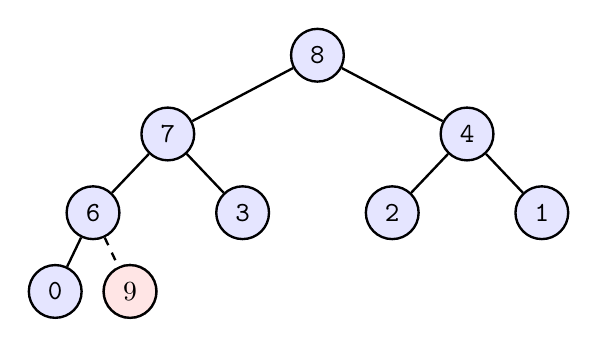
\begin{tikzpicture}

\fill[blue!10] (0.0, 0.0) circle (0.35);
\node [line width=0.03cm,black,minimum size=0.6699999999999999cm,draw,circle] at (0.0,0.0)(8){};\draw (0.0, 0.0) node[color=black] {\texttt{8}};
\fill[blue!10] (-1.9, -1.0) circle (0.35);
\node [line width=0.03cm,black,minimum size=0.6699999999999999cm,draw,circle] at (-1.9,-1.0)(7){};\draw (-1.9, -1.0) node[color=black] {\texttt{7}};
\fill[blue!10] (1.9, -1.0) circle (0.35);
\node [line width=0.03cm,black,minimum size=0.6699999999999999cm,draw,circle] at (1.9,-1.0)(4){};\draw (1.9, -1.0) node[color=black] {\texttt{4}};
\fill[blue!10] (-2.85, -2.0) circle (0.35);
\node [line width=0.03cm,black,minimum size=0.6699999999999999cm,draw,circle] at (-2.85,-2.0)(6){};\draw (-2.85, -2.0) node[color=black] {\texttt{6}};
\fill[blue!10] (-0.95, -2.0) circle (0.35);
\node [line width=0.03cm,black,minimum size=0.6699999999999999cm,draw,circle] at (-0.95,-2.0)(3){};\draw (-0.95, -2.0) node[color=black] {\texttt{3}};
\fill[blue!10] (0.95, -2.0) circle (0.35);
\node [line width=0.03cm,black,minimum size=0.6699999999999999cm,draw,circle] at (0.95,-2.0)(2){};\draw (0.95, -2.0) node[color=black] {\texttt{2}};
\fill[blue!10] (2.85, -2.0) circle (0.35);
\node [line width=0.03cm,black,minimum size=0.6699999999999999cm,draw,circle] at (2.85,-2.0)(1){};\draw (2.85, -2.0) node[color=black] {\texttt{1}};
\fill[blue!10] (-3.33, -3.0) circle (0.35);
\node [line width=0.03cm,black,minimum size=0.6699999999999999cm,draw,circle] at (-3.33,-3.0)(0){};\draw (-3.33, -3.0) node[color=black] {\texttt{0}};
\fill[blue!10] (-2.38, -3.0) circle (0.35);
\node [line width=0.03cm,black,minimum size=0.6699999999999999cm,draw,circle] at (-2.38,-3.0)(9){};\draw (-2.38, -3.0) node[color=black] {\texttt{9}};\draw[line width=0.03cm,black] (8) to  (7);
\draw[line width=0.03cm,black] (8) to  (4);
\draw[line width=0.03cm,black] (7) to  (6);
\draw[line width=0.03cm,black] (7) to  (3);
\draw[line width=0.03cm,black] (4) to  (2);
\draw[line width=0.03cm,black] (4) to  (1);
\draw[line width=0.03cm,black] (6) to  (0);
\draw[line width=0.03cm,black] (6) to  (9);

\fill[red!10] (-2.38, -3.0) circle (0.35);
\draw[line width=0.03cm,black] (-2.38, -3.0) circle (0.33499999999999996);\draw (-2.38, -3.0) node[color=black] {9};\draw[line width=0.1cm,white] (6) to  (9);
\draw[line width=0.03cm,black,,dashed] (6) to  (9);
\end{tikzpicture}

\end{center}



(c): I cannot perform a left rotation on $T$ about
node 4 because 4 does not have a right child.

(d):
When I perform a right rotation on $T$ about node \verb!4! I get:
\begin{center}
\begin{tikzpicture}

\fill[white] (13.0, -3.0) circle (0.3);
\node [line width=0.03cm,black,minimum size=0.57cm,draw,circle] at (13.0,-3.0)(h){};\draw (13.0, -3.0) node[color=black] {\texttt{19}};
\fill[white] (15.0, -3.0) circle (0.3);
\node [line width=0.03cm,black,minimum size=0.57cm,draw,circle] at (15.0,-3.0)(m){};\draw (15.0, -3.0) node[color=black] {\texttt{26}};
\fill[white] (5.0, 0.0) circle (0.3);
\node [draw=none,line width=0cm,black,minimum size=0.6cm,circle] at (5.0,0.0)(X){};
\fill[white] (17.0, 0.0) circle (0.3);
\node [draw=none,line width=0cm,black,minimum size=0.6cm,circle] at (17.0,0.0)(Y){};
\fill[white] (11.0, 0.0) circle (0.3);
\node [line width=0.03cm,black,minimum size=0.57cm,draw,circle] at (11.0,0.0)(a){};\draw (11.0, 0.0) node[color=black] {\texttt{10}};
\fill[white] (9.0, -1.0) circle (0.3);
\node [line width=0.03cm,black,minimum size=0.57cm,draw,circle] at (9.0,-1.0)(b){};\draw (9.0, -1.0) node[color=black] {\texttt{2}};
\fill[white] (14.0, -2.0) circle (0.3);
\node [line width=0.03cm,black,minimum size=0.57cm,draw,circle] at (14.0,-2.0)(d){};\draw (14.0, -2.0) node[color=black] {\texttt{20}};
\fill[white] (8.0, -2.0) circle (0.3);
\node [line width=0.03cm,black,minimum size=0.57cm,draw,circle] at (8.0,-2.0)(e){};\draw (8.0, -2.0) node[color=black] {\texttt{0}};
\fill[white] (12.0, -2.0) circle (0.3);
\node [line width=0.03cm,black,minimum size=0.57cm,draw,circle] at (12.0,-2.0)(f){};\draw (12.0, -2.0) node[color=black] {\texttt{17}};
\fill[white] (9.0, -3.0) circle (0.3);
\node [line width=0.03cm,black,minimum size=0.57cm,draw,circle] at (9.0,-3.0)(k){};\draw (9.0, -3.0) node[color=black] {\texttt{3}};
\fill[white] (10.0, -2.0) circle (0.3);
\node [line width=0.03cm,black,minimum size=0.57cm,draw,circle] at (10.0,-2.0)(l){};\draw (10.0, -2.0) node[color=black] {\texttt{4}};
\fill[white] (13.0, -1.0) circle (0.3);
\node [line width=0.03cm,black,minimum size=0.57cm,draw,circle] at (13.0,-1.0)(p){};\draw (13.0, -1.0) node[color=black] {\texttt{18}};\draw[line width=0.03cm,black,->,>=triangle 60] (l) to  (k);
\draw[line width=0.03cm,black,->,>=triangle 60] (p) to  (f);
\draw[line width=0.03cm,black,->,>=triangle 60] (p) to  (d);
\draw[line width=0.03cm,black,->,>=triangle 60] (a) to  (p);
\draw[line width=0.03cm,black,->,>=triangle 60] (a) to  (b);
\draw[line width=0.03cm,black,->,>=triangle 60] (b) to  (e);
\draw[line width=0.03cm,black,->,>=triangle 60] (b) to  (l);
\draw[line width=0.03cm,black,->,>=triangle 60] (d) to  (h);
\draw[line width=0.03cm,black,->,>=triangle 60] (d) to  (m);
\end{tikzpicture}

\end{center}



(e): Perform a left rotation at 18.

(f): Perform a right rotation at 18.

(g): Perform a left rotation at 2.

(h): Perform a right rotation at 2.

(i): Why can't you perform a left rotation at 17?

(j): Why can't you perform a right rotation at 17?

(k): Perform a left rotation at 20.

(l): Perform a right rotation at 20.

\end{eg}

\newpage
\begin{ex}
  You are given the following BST $T$:
  \begin{center}
\begin{tikzpicture}

\fill[white] (0.0, 0.0) circle (0.3);
\node [line width=0.03cm,black,minimum size=0.57cm,draw,circle] at (0.0,0.0)(14){};\draw (0.0, 0.0) node[color=black] {\texttt{14}};
\fill[white] (-3.2, -1.0) circle (0.3);
\node [line width=0.03cm,black,minimum size=0.57cm,draw,circle] at (-3.2,-1.0)(9){};\draw (-3.2, -1.0) node[color=black] {\texttt{9}};
\fill[white] (3.2, -1.0) circle (0.3);
\node [line width=0.03cm,black,minimum size=0.57cm,draw,circle] at (3.2,-1.0)(18){};\draw (3.2, -1.0) node[color=black] {\texttt{18}};
\fill[white] (-4.8, -2.0) circle (0.3);
\node [line width=0.03cm,black,minimum size=0.57cm,draw,circle] at (-4.8,-2.0)(5){};\draw (-4.8, -2.0) node[color=black] {\texttt{5}};
\fill[white] (-1.6, -2.0) circle (0.3);
\node [line width=0.03cm,black,minimum size=0.57cm,draw,circle] at (-1.6,-2.0)(13){};\draw (-1.6, -2.0) node[color=black] {\texttt{13}};
\fill[white] (1.6, -2.0) circle (0.3);
\node [line width=0.03cm,black,minimum size=0.57cm,draw,circle] at (1.6,-2.0)(15){};\draw (1.6, -2.0) node[color=black] {\texttt{15}};
\fill[white] (4.8, -2.0) circle (0.3);
\node [line width=0.03cm,black,minimum size=0.57cm,draw,circle] at (4.8,-2.0)(22){};\draw (4.8, -2.0) node[color=black] {\texttt{22}};
\fill[white] (-5.6, -3.0) circle (0.3);
\node [line width=0.03cm,black,minimum size=0.57cm,draw,circle] at (-5.6,-3.0)(0){};\draw (-5.6, -3.0) node[color=black] {\texttt{0}};
\fill[white] (-4.0, -3.0) circle (0.3);
\node [line width=0.03cm,black,minimum size=0.57cm,draw,circle] at (-4.0,-3.0)(8){};\draw (-4.0, -3.0) node[color=black] {\texttt{8}};
\fill[white] (-2.4, -3.0) circle (0.3);
\node [line width=0.03cm,black,minimum size=0.57cm,draw,circle] at (-2.4,-3.0)(10){};\draw (-2.4, -3.0) node[color=black] {\texttt{10}};
\fill[white] (4.0, -3.0) circle (0.3);
\node [line width=0.03cm,black,minimum size=0.57cm,draw,circle] at (4.0,-3.0)(21){};\draw (4.0, -3.0) node[color=black] {\texttt{21}};
\fill[white] (5.6, -3.0) circle (0.3);
\node [line width=0.03cm,black,minimum size=0.57cm,draw,circle] at (5.6,-3.0)(31){};\draw (5.6, -3.0) node[color=black] {\texttt{31}};
\fill[white] (-4.4, -4.0) circle (0.3);
\node [line width=0.03cm,black,minimum size=0.57cm,draw,circle] at (-4.4,-4.0)(7){};\draw (-4.4, -4.0) node[color=black] {\texttt{7}};
\fill[white] (-2.0, -4.0) circle (0.3);
\node [line width=0.03cm,black,minimum size=0.57cm,draw,circle] at (-2.0,-4.0)(11){};\draw (-2.0, -4.0) node[color=black] {\texttt{11}};
\fill[white] (3.6, -4.0) circle (0.3);
\node [line width=0.03cm,black,minimum size=0.57cm,draw,circle] at (3.6,-4.0)(19){};\draw (3.6, -4.0) node[color=black] {\texttt{19}};\draw[line width=0.03cm,black,->,>=triangle 60] (14) to  (9);
\draw[line width=0.03cm,black,->,>=triangle 60] (14) to  (18);
\draw[line width=0.03cm,black,->,>=triangle 60] (9) to  (5);
\draw[line width=0.03cm,black,->,>=triangle 60] (9) to  (13);
\draw[line width=0.03cm,black,->,>=triangle 60] (18) to  (15);
\draw[line width=0.03cm,black,->,>=triangle 60] (18) to  (22);
\draw[line width=0.03cm,black,->,>=triangle 60] (5) to  (0);
\draw[line width=0.03cm,black,->,>=triangle 60] (5) to  (8);
\draw[line width=0.03cm,black,->,>=triangle 60] (13) to  (10);
\draw[line width=0.03cm,black,->,>=triangle 60] (22) to  (21);
\draw[line width=0.03cm,black,->,>=triangle 60] (22) to  (31);
\draw[line width=0.03cm,black,->,>=triangle 60] (8) to  (7);
\draw[line width=0.03cm,black,->,>=triangle 60] (10) to  (11);
\draw[line width=0.03cm,black,->,>=triangle 60] (21) to  (19);
\end{tikzpicture}

\end{center}


  
Perform left and right rotation at every node of $T$ whenever possible.
[For instance you cannot left nor right rotate at 0; you cannot left rotate at 8, but you can right rotate at 8.] 
\end{ex}



\newpage
\subsection{Algorithms for left and right rotations}

Here are the algorithms for the left and right rotations.

{\small
\begin{console}
ALGORITHM: LEFT ROTATION
INPUT    : p

/* We want to perform left rotation about node (a). p points
to (a). From
                   ...
                    |
            p----> (a)
                   / \
                 T1  (b) <-----q
                     / \
                   T2   T3
we want to obtain this:
                    ...
                     |
                    (b) <-----q
                    / \
           p----> (a)  T3
                  / \
                 T1  T2
Note that we assume p and q are not NULL.
*/

    Node * q = p->right()

    // Move (a) down and (b) up
    q->parent_ = p->parent_  
    p->parent_ = q           

    // Move T2 from (b) to (a)
    p->right_ = q->left_    
    q->left_ = p
\end{console}
}

{\small
\begin{console}
ALGORITHM: RIGHT-ROTATION
INPUT    : p

/* We want to perform right rotation about node (a). p points
to (a). From
                   ...
                    |
                   (a) <----p
                   / \
          q----> (b)  T3 
                 / \
               T1   T2

we want to obtain
                    ...
                     |
              q---> (b)
                    / \
                  T1  (a) <----p
                      / \   
                    T2   T3

Note that we assume p and q are not NULL.
*/

    Node * q = p->left_;

    // Move (a) down and (b) up
    q->parent_ = p->parent_;  
    p->parent_ = q;           

    // Move T2 from (b) to (a)
    p->left_ = q->right_;   
    q->right_ = p;
\end{console}
}

\newpage
\subsection{Using rotations to balance BST}

Suppose I have this BST:
\begin{center}
\begin{tikzpicture}

\fill[white] (0.0, 0.0) circle (0.3);
\node [line width=0.03cm,black,minimum size=0.57cm,draw,circle] at (0.0,0.0)(10){};\draw (0.0, 0.0) node[color=black] {\texttt{10}};
\fill[white] (-3.0, -1.0) circle (0.3);
\node [line width=0.03cm,black,minimum size=0.57cm,draw,circle] at (-3.0,-1.0)(4){};\draw (-3.0, -1.0) node[color=black] {\texttt{4}};
\fill[white] (3.0, -1.0) circle (0.3);
\node [line width=0.03cm,black,minimum size=0.57cm,draw,circle] at (3.0,-1.0)(18){};\draw (3.0, -1.0) node[color=black] {\texttt{18}};
\fill[white] (-4.5, -2.0) circle (0.3);
\node [line width=0.03cm,black,minimum size=0.57cm,draw,circle] at (-4.5,-2.0)(2){};\draw (-4.5, -2.0) node[color=black] {\texttt{2}};
\fill[white] (1.5, -2.0) circle (0.3);
\node [line width=0.03cm,black,minimum size=0.57cm,draw,circle] at (1.5,-2.0)(17){};\draw (1.5, -2.0) node[color=black] {\texttt{17}};
\fill[white] (4.5, -2.0) circle (0.3);
\node [line width=0.03cm,black,minimum size=0.57cm,draw,circle] at (4.5,-2.0)(20){};\draw (4.5, -2.0) node[color=black] {\texttt{20}};
\fill[white] (-5.25, -3.0) circle (0.3);
\node [line width=0.03cm,black,minimum size=0.57cm,draw,circle] at (-5.25,-3.0)(0){};\draw (-5.25, -3.0) node[color=black] {\texttt{0}};
\fill[white] (-3.75, -3.0) circle (0.3);
\node [line width=0.03cm,black,minimum size=0.57cm,draw,circle] at (-3.75,-3.0)(3){};\draw (-3.75, -3.0) node[color=black] {\texttt{3}};\draw[line width=0.03cm,black,->,>=triangle 60] (10) to  (4);
\draw[line width=0.03cm,black,->,>=triangle 60] (10) to  (18);
\draw[line width=0.03cm,black,->,>=triangle 60] (4) to  (2);
\draw[line width=0.03cm,black,->,>=triangle 60] (18) to  (17);
\draw[line width=0.03cm,black,->,>=triangle 60] (18) to  (20);
\draw[line width=0.03cm,black,->,>=triangle 60] (2) to  (0);
\draw[line width=0.03cm,black,->,>=triangle 60] (2) to  (3);
\end{tikzpicture}

\end{center}



The tree is clearly not balanced at \verb!4!: the left height us 1
and the right height is -1.
I'm going to perform a left rotation about \verb!4!:
\begin{center}
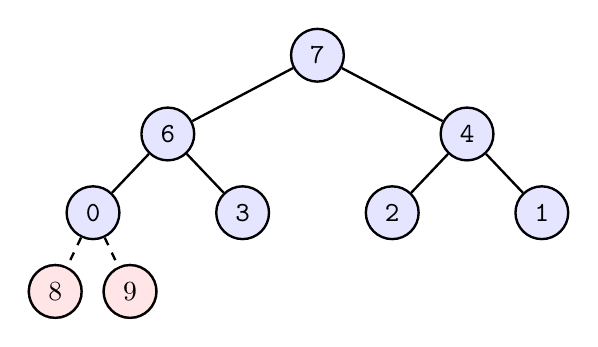
\begin{tikzpicture}

\fill[blue!10] (0.0, 0.0) circle (0.35);
\node [line width=0.03cm,black,minimum size=0.6699999999999999cm,draw,circle] at (0.0,0.0)(7){};\draw (0.0, 0.0) node[color=black] {\texttt{7}};
\fill[blue!10] (-1.9, -1.0) circle (0.35);
\node [line width=0.03cm,black,minimum size=0.6699999999999999cm,draw,circle] at (-1.9,-1.0)(6){};\draw (-1.9, -1.0) node[color=black] {\texttt{6}};
\fill[blue!10] (1.9, -1.0) circle (0.35);
\node [line width=0.03cm,black,minimum size=0.6699999999999999cm,draw,circle] at (1.9,-1.0)(4){};\draw (1.9, -1.0) node[color=black] {\texttt{4}};
\fill[blue!10] (-2.85, -2.0) circle (0.35);
\node [line width=0.03cm,black,minimum size=0.6699999999999999cm,draw,circle] at (-2.85,-2.0)(0){};\draw (-2.85, -2.0) node[color=black] {\texttt{0}};
\fill[blue!10] (-0.95, -2.0) circle (0.35);
\node [line width=0.03cm,black,minimum size=0.6699999999999999cm,draw,circle] at (-0.95,-2.0)(3){};\draw (-0.95, -2.0) node[color=black] {\texttt{3}};
\fill[blue!10] (0.95, -2.0) circle (0.35);
\node [line width=0.03cm,black,minimum size=0.6699999999999999cm,draw,circle] at (0.95,-2.0)(2){};\draw (0.95, -2.0) node[color=black] {\texttt{2}};
\fill[blue!10] (2.85, -2.0) circle (0.35);
\node [line width=0.03cm,black,minimum size=0.6699999999999999cm,draw,circle] at (2.85,-2.0)(1){};\draw (2.85, -2.0) node[color=black] {\texttt{1}};
\fill[blue!10] (-3.33, -3.0) circle (0.35);
\node [line width=0.03cm,black,minimum size=0.6699999999999999cm,draw,circle] at (-3.33,-3.0)(8){};\draw (-3.33, -3.0) node[color=black] {\texttt{8}};
\fill[blue!10] (-2.38, -3.0) circle (0.35);
\node [line width=0.03cm,black,minimum size=0.6699999999999999cm,draw,circle] at (-2.38,-3.0)(9){};\draw (-2.38, -3.0) node[color=black] {\texttt{9}};\draw[line width=0.03cm,black] (7) to  (6);
\draw[line width=0.03cm,black] (7) to  (4);
\draw[line width=0.03cm,black] (6) to  (0);
\draw[line width=0.03cm,black] (6) to  (3);
\draw[line width=0.03cm,black] (4) to  (2);
\draw[line width=0.03cm,black] (4) to  (1);
\draw[line width=0.03cm,black] (0) to  (8);
\draw[line width=0.03cm,black] (0) to  (9);

\fill[red!10] (-2.38, -3.0) circle (0.35);
\draw[line width=0.03cm,black] (-2.38, -3.0) circle (0.33499999999999996);\draw (-2.38, -3.0) node[color=black] {9};
\fill[red!10] (-3.33, -3.0) circle (0.35);
\draw[line width=0.03cm,black] (-3.33, -3.0) circle (0.33499999999999996);\draw (-3.33, -3.0) node[color=black] {8};\draw[line width=0.1cm,white] (0) to  (9);
\draw[line width=0.03cm,black,,dashed] (0) to  (9);
\draw[line width=0.1cm,white] (0) to  (8);
\draw[line width=0.03cm,black,,dashed] (0) to  (8);
\end{tikzpicture}

\end{center}




Note that the tree is now height--balanced.


\newpage
\subsection{Height changes due to rotations}

Now let's analyze the general case.

Let $T$ be the subtree tree with root $\alpha$
before the rotation and $\operatorname{LEFT}(T)$
be this subtree after.
The following are the relevant heights before and after
left rotation about node $\alpha$:
\begin{align*}
  \operatorname{height}(T) &=
  1 +
  \max(\operatorname{height}(T_1),
  1 + \max(\operatorname{height}(T_2), \operatorname{height}(T_3)))
  \\
  \operatorname{height}(\operatorname{LEFT}(T)) &=
  1 + \max(1+\max(\operatorname{height}(T_1),\operatorname{height}(T_2)),
  \operatorname{height}(T_3)))
\end{align*}
or, to make it easier to read, if I write $h_i$ for
$\operatorname{height}(T_i)$, then
\begin{align*}
  \operatorname{height}(T) &=
  1 +
  \max(h_1,
  1 + \max(h_2, h_3))
  \\
  \operatorname{height}(\operatorname{LEFT}(T)) &=
  1 + \max(1+\max(h_1,h_2),h_3)
\end{align*}
So it the heights are $h_1=2, h_2=1, h_3=3$, then
\begin{align*}
  \operatorname{height}(T) &=
  1 +
  \max(2,
  1 + \max(1, 3)) = 1 + \max(2, 4)
  \\
  \operatorname{height}(\operatorname{LEFT}(T)) &=
  1 + \max(1+\max(2,1),3)
  = 1 + \max(3, 3)
\end{align*}
For the pre-left-rotation case, you see that the two subtrees of $\alpha$
have
heights 2 and 4 and is therefore unbalanced.
After rotation, the two subtrees of $\beta$ has heights $3$ and $3$ is
balanced.


Suppose you have added a node with value $k$ into a BST
and it become unbalanced.
It should be clear unbalanced nodes (if any)
must be along the path that $k$ takes within the tree
as it finds its place of insertion.
When you go from the inserted new node back to the root,
suppose the first node that is unbalanced is $\alpha$:
\begin{center}
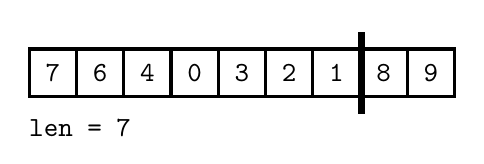
\begin{tikzpicture}

\draw (0.3, -0.3)
  node[draw, line width=0.04cm, , color=black,
       rounded corners=0cm, inner sep=0cm] {

\begin{minipage}[t][0.6cm]{0.6cm}
\mbox{}

\end{minipage}

};\draw (0.3, -0.3) node[color=black] {{\texttt{7}}};
\draw (0.8999999999999999, -0.3)
  node[draw, line width=0.04cm, , color=black,
       rounded corners=0cm, inner sep=0cm] {

\begin{minipage}[t][0.6cm]{0.6cm}
\mbox{}

\end{minipage}

};\draw (0.8999999999999999, -0.3) node[color=black] {{\texttt{6}}};
\draw (1.5, -0.3)
  node[draw, line width=0.04cm, , color=black,
       rounded corners=0cm, inner sep=0cm] {

\begin{minipage}[t][0.6cm]{0.6cm}
\mbox{}

\end{minipage}

};\draw (1.5, -0.3) node[color=black] {{\texttt{4}}};
\draw (2.0999999999999996, -0.3)
  node[draw, line width=0.04cm, , color=black,
       rounded corners=0cm, inner sep=0cm] {

\begin{minipage}[t][0.6cm]{0.6cm}
\mbox{}

\end{minipage}

};\draw (2.0999999999999996, -0.3) node[color=black] {{\texttt{0}}};
\draw (2.7, -0.3)
  node[draw, line width=0.04cm, , color=black,
       rounded corners=0cm, inner sep=0cm] {

\begin{minipage}[t][0.6cm]{0.6cm}
\mbox{}

\end{minipage}

};\draw (2.7, -0.3) node[color=black] {{\texttt{3}}};
\draw (3.3, -0.3)
  node[draw, line width=0.04cm, , color=black,
       rounded corners=0cm, inner sep=0cm] {

\begin{minipage}[t][0.6cm]{0.6cm}
\mbox{}

\end{minipage}

};\draw (3.3, -0.3) node[color=black] {{\texttt{2}}};
\draw (3.9, -0.3)
  node[draw, line width=0.04cm, , color=black,
       rounded corners=0cm, inner sep=0cm] {

\begin{minipage}[t][0.6cm]{0.6cm}
\mbox{}

\end{minipage}

};\draw (3.9, -0.3) node[color=black] {{\texttt{1}}};
\draw (4.5, -0.3)
  node[draw, line width=0.04cm, , color=black,
       rounded corners=0cm, inner sep=0cm] {

\begin{minipage}[t][0.6cm]{0.6cm}
\mbox{}

\end{minipage}

};\draw (4.5, -0.3) node[color=black] {{\texttt{8}}};
\draw (5.1, -0.3)
  node[draw, line width=0.04cm, , color=black,
       rounded corners=0cm, inner sep=0cm] {

\begin{minipage}[t][0.6cm]{0.6cm}
\mbox{}

\end{minipage}

};\draw (5.1, -0.3) node[color=black] {{\texttt{9}}};\draw[line width=0.1cm,black] (4.22,-0.82) to  (4.22,0.22);

\draw (1.0, -1.0)
  node[draw=none, line width=0cm, , color=black,
       rounded corners=0cm, inner sep=0cm] {

\begin{minipage}[t][0.1cm]{2cm}
\mbox{}

\end{minipage}

};
\draw (1.0, -1.0) node[color=black,
 inner sep=0cm] {
 
\begin{minipage}[t][0.1cm]{2cm}
\texttt{len = 7}
\end{minipage}

};
\end{tikzpicture}

\end{center}



\underline{CASE LEFT: 
$k$ is inserted into the left subtree of $\alpha$.}

\begin{center}

\begin{tikzpicture}
\node at (3,-0.8) [minimum size=8mm] (E) {$$};
\node at (2,-2.4000000000000004) [circle,draw,minimum size=8mm] (A) {$\alpha$};
\node at (0,-3.2)
    [isosceles triangle, shape border rotate=+90,
     draw,minimum size=8mm,minimum height=2cm,
     anchor=north] (Ctriangle) {$T_1+k$};
\coordinate (C) at (0,-3.2);
\node at (4,-3.2)
    [isosceles triangle, shape border rotate=+90,
     draw,minimum size=8mm,minimum height=2cm,
     anchor=north] (Btriangle) {$T_2$};
\coordinate (B) at (4,-3.2);
\draw [-,thick] (A) -- (B);
\draw [-,thick] (A) -- (C);
\draw [-,thick] (E) -- (A);

;
\end{tikzpicture}
    
\end{center}


Of course before adding $k$, $\alpha$ is balanced:
\[
h(T_1) = h(T_2) + \ep
\]
where $\ep = -1, 0, 1$.
Since $\alpha$ is unbalanced  after adding $k$, we must have
\[
h(T_1 + k) = h(T_2) + 2
\]
(the 2 on the right can't be more than 2, right?)
and 
\[
h(T_1) = h(T_2) + 1
\]
This implies that $T_1$ must have at least one node.
So let me draw the tree, before inserting $k$, at $\alpha$ like this:
\begin{center}
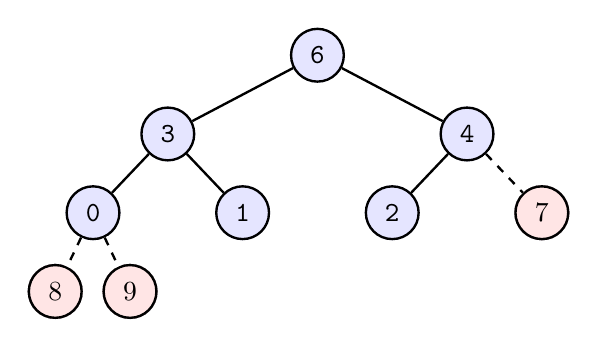
\begin{tikzpicture}

\fill[blue!10] (0.0, 0.0) circle (0.35);
\node [line width=0.03cm,black,minimum size=0.6699999999999999cm,draw,circle] at (0.0,0.0)(6){};\draw (0.0, 0.0) node[color=black] {\texttt{6}};
\fill[blue!10] (-1.9, -1.0) circle (0.35);
\node [line width=0.03cm,black,minimum size=0.6699999999999999cm,draw,circle] at (-1.9,-1.0)(3){};\draw (-1.9, -1.0) node[color=black] {\texttt{3}};
\fill[blue!10] (1.9, -1.0) circle (0.35);
\node [line width=0.03cm,black,minimum size=0.6699999999999999cm,draw,circle] at (1.9,-1.0)(4){};\draw (1.9, -1.0) node[color=black] {\texttt{4}};
\fill[blue!10] (-2.85, -2.0) circle (0.35);
\node [line width=0.03cm,black,minimum size=0.6699999999999999cm,draw,circle] at (-2.85,-2.0)(0){};\draw (-2.85, -2.0) node[color=black] {\texttt{0}};
\fill[blue!10] (-0.95, -2.0) circle (0.35);
\node [line width=0.03cm,black,minimum size=0.6699999999999999cm,draw,circle] at (-0.95,-2.0)(1){};\draw (-0.95, -2.0) node[color=black] {\texttt{1}};
\fill[blue!10] (0.95, -2.0) circle (0.35);
\node [line width=0.03cm,black,minimum size=0.6699999999999999cm,draw,circle] at (0.95,-2.0)(2){};\draw (0.95, -2.0) node[color=black] {\texttt{2}};
\fill[blue!10] (2.85, -2.0) circle (0.35);
\node [line width=0.03cm,black,minimum size=0.6699999999999999cm,draw,circle] at (2.85,-2.0)(7){};\draw (2.85, -2.0) node[color=black] {\texttt{7}};
\fill[blue!10] (-3.33, -3.0) circle (0.35);
\node [line width=0.03cm,black,minimum size=0.6699999999999999cm,draw,circle] at (-3.33,-3.0)(8){};\draw (-3.33, -3.0) node[color=black] {\texttt{8}};
\fill[blue!10] (-2.38, -3.0) circle (0.35);
\node [line width=0.03cm,black,minimum size=0.6699999999999999cm,draw,circle] at (-2.38,-3.0)(9){};\draw (-2.38, -3.0) node[color=black] {\texttt{9}};\draw[line width=0.03cm,black] (6) to  (3);
\draw[line width=0.03cm,black] (6) to  (4);
\draw[line width=0.03cm,black] (3) to  (0);
\draw[line width=0.03cm,black] (3) to  (1);
\draw[line width=0.03cm,black] (4) to  (2);
\draw[line width=0.03cm,black] (4) to  (7);
\draw[line width=0.03cm,black] (0) to  (8);
\draw[line width=0.03cm,black] (0) to  (9);

\fill[red!10] (-2.38, -3.0) circle (0.35);
\draw[line width=0.03cm,black] (-2.38, -3.0) circle (0.33499999999999996);\draw (-2.38, -3.0) node[color=black] {9};
\fill[red!10] (-3.33, -3.0) circle (0.35);
\draw[line width=0.03cm,black] (-3.33, -3.0) circle (0.33499999999999996);\draw (-3.33, -3.0) node[color=black] {8};
\fill[red!10] (2.85, -2.0) circle (0.35);
\draw[line width=0.03cm,black] (2.85, -2.0) circle (0.33499999999999996);\draw (2.85, -2.0) node[color=black] {7};\draw[line width=0.1cm,white] (0) to  (9);
\draw[line width=0.03cm,black,,dashed] (0) to  (9);
\draw[line width=0.1cm,white] (0) to  (8);
\draw[line width=0.03cm,black,,dashed] (0) to  (8);
\draw[line width=0.1cm,white] (4) to  (7);
\draw[line width=0.03cm,black,,dashed] (4) to  (7);
\end{tikzpicture}

\end{center}


Tying this to the previous diagram, 
we have
\[
1 + \max(h(T'_1), h(T'_2)) = h(T'_3) + 1
\]
i.e., 
\[
\max(h(T'_1), h(T'_2)) = h(T'_3)
\]

\underline{CASE LEFT-LEFT: $k$ is inserted into the 
left subtree of the left subtree of $\alpha$.}
Here's the picture:

\begin{center}

\begin{tikzpicture}
\node at (4,-0.8) [minimum size=8mm] (E) {$$};
\node at (3,-2.4000000000000004) [circle,draw,minimum size=8mm] (A) {$\alpha$};
\node at (1,-3.2) [circle,draw,minimum size=8mm] (C) {$\beta$};
\node at (5,-3.2)
    [isosceles triangle, shape border rotate=+90,
     draw,minimum size=8mm,
     anchor=north] (Btriangle) {$T'_3$};
\coordinate (B) at (5,-3.2);
\node at (0,-4.0)
    [isosceles triangle, shape border rotate=+90,
     draw,minimum size=8mm,
     anchor=north] (Dtriangle) {$T'_1+k$};
\coordinate (D) at (0,-4.0);
\node at (2,-4.0)
    [isosceles triangle, shape border rotate=+90,
     draw,minimum size=8mm,
     anchor=north] (Ftriangle) {$T'_2$};
\coordinate (F) at (2,-4.0);
\draw [-,thick] (A) -- (B);
\draw [-,thick] (A) -- (C);
\draw [-,thick] (E) -- (A);
\draw [-,thick] (C) -- (D);
\draw [-,thick] (C) -- (F);

;
\end{tikzpicture}
    
\end{center}


I claim that
\[
h(T'_1) = h(T'_2) = h(T'_3) 
\]


By our assumption, this makes the tree unbalanced by $\alpha$.
We had this before adding $k$:
\[
\max(h(T'_1), h(T'_2)) = h(T'_3)
\]
On adding $k$ for this case, i.e., to $T_1'$, 
$\alpha$ becomes unbalanced.
Therefore
\[
h(T'_1 + k) = h(T'_1) + 1,
\,\,\,\,\,
h(T'_1) \geq h(T'_2)
\]
That means that 
\[
h(T'_1) = h(T'_3)
\]
Note also that if $h(T'_1) > h(T'_2)$,
then when $k$ is added to $T'_1$, the resulting
tree is unbalanced at $\beta$
which contradicts out assumption that 
the resulting tree is unbalanced at $\alpha$.
Hence we must have $h(T'_1) = h(T'_2)$.
Altogether we have 
\[
h(T'_1) = h(T'_2) = h(T'_3)
\] 

I right--rotate at $\alpha$ to get this:
\begin{center}
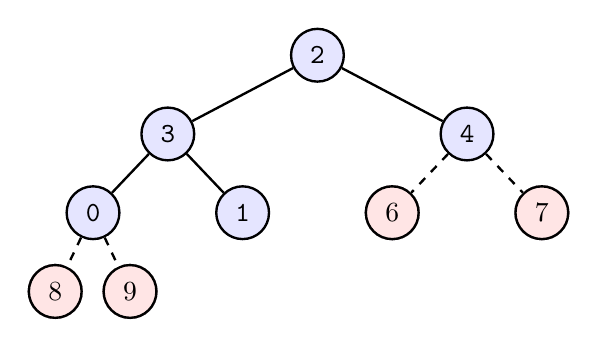
\begin{tikzpicture}

\fill[blue!10] (0.0, 0.0) circle (0.35);
\node [line width=0.03cm,black,minimum size=0.6699999999999999cm,draw,circle] at (0.0,0.0)(2){};\draw (0.0, 0.0) node[color=black] {\texttt{2}};
\fill[blue!10] (-1.9, -1.0) circle (0.35);
\node [line width=0.03cm,black,minimum size=0.6699999999999999cm,draw,circle] at (-1.9,-1.0)(3){};\draw (-1.9, -1.0) node[color=black] {\texttt{3}};
\fill[blue!10] (1.9, -1.0) circle (0.35);
\node [line width=0.03cm,black,minimum size=0.6699999999999999cm,draw,circle] at (1.9,-1.0)(4){};\draw (1.9, -1.0) node[color=black] {\texttt{4}};
\fill[blue!10] (-2.85, -2.0) circle (0.35);
\node [line width=0.03cm,black,minimum size=0.6699999999999999cm,draw,circle] at (-2.85,-2.0)(0){};\draw (-2.85, -2.0) node[color=black] {\texttt{0}};
\fill[blue!10] (-0.95, -2.0) circle (0.35);
\node [line width=0.03cm,black,minimum size=0.6699999999999999cm,draw,circle] at (-0.95,-2.0)(1){};\draw (-0.95, -2.0) node[color=black] {\texttt{1}};
\fill[blue!10] (0.95, -2.0) circle (0.35);
\node [line width=0.03cm,black,minimum size=0.6699999999999999cm,draw,circle] at (0.95,-2.0)(6){};\draw (0.95, -2.0) node[color=black] {\texttt{6}};
\fill[blue!10] (2.85, -2.0) circle (0.35);
\node [line width=0.03cm,black,minimum size=0.6699999999999999cm,draw,circle] at (2.85,-2.0)(7){};\draw (2.85, -2.0) node[color=black] {\texttt{7}};
\fill[blue!10] (-3.33, -3.0) circle (0.35);
\node [line width=0.03cm,black,minimum size=0.6699999999999999cm,draw,circle] at (-3.33,-3.0)(8){};\draw (-3.33, -3.0) node[color=black] {\texttt{8}};
\fill[blue!10] (-2.38, -3.0) circle (0.35);
\node [line width=0.03cm,black,minimum size=0.6699999999999999cm,draw,circle] at (-2.38,-3.0)(9){};\draw (-2.38, -3.0) node[color=black] {\texttt{9}};\draw[line width=0.03cm,black] (2) to  (3);
\draw[line width=0.03cm,black] (2) to  (4);
\draw[line width=0.03cm,black] (3) to  (0);
\draw[line width=0.03cm,black] (3) to  (1);
\draw[line width=0.03cm,black] (4) to  (6);
\draw[line width=0.03cm,black] (4) to  (7);
\draw[line width=0.03cm,black] (0) to  (8);
\draw[line width=0.03cm,black] (0) to  (9);

\fill[red!10] (-2.38, -3.0) circle (0.35);
\draw[line width=0.03cm,black] (-2.38, -3.0) circle (0.33499999999999996);\draw (-2.38, -3.0) node[color=black] {9};
\fill[red!10] (-3.33, -3.0) circle (0.35);
\draw[line width=0.03cm,black] (-3.33, -3.0) circle (0.33499999999999996);\draw (-3.33, -3.0) node[color=black] {8};
\fill[red!10] (2.85, -2.0) circle (0.35);
\draw[line width=0.03cm,black] (2.85, -2.0) circle (0.33499999999999996);\draw (2.85, -2.0) node[color=black] {7};
\fill[red!10] (0.95, -2.0) circle (0.35);
\draw[line width=0.03cm,black] (0.95, -2.0) circle (0.33499999999999996);\draw (0.95, -2.0) node[color=black] {6};\draw[line width=0.1cm,white] (0) to  (9);
\draw[line width=0.03cm,black,,dashed] (0) to  (9);
\draw[line width=0.1cm,white] (0) to  (8);
\draw[line width=0.03cm,black,,dashed] (0) to  (8);
\draw[line width=0.1cm,white] (4) to  (7);
\draw[line width=0.03cm,black,,dashed] (4) to  (7);
\draw[line width=0.1cm,white] (4) to  (6);
\draw[line width=0.03cm,black,,dashed] (4) to  (6);
\end{tikzpicture}

\end{center}


The height of the left subtree of $\beta$ is $h(T'_1) + 1$
and the height of the right subtree at 
$\beta$ is $1 + \max(h(T'_2), h(T'_3)) = 1 + h(T'_1)$.
Therefore this resulting tree is balanced at $\beta$.

Note for the original tree, before inserting $k$
and when the tree was balanced,
\begin{center}
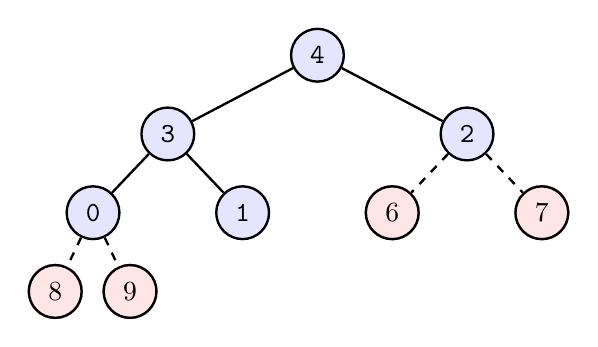
\begin{tikzpicture}

\fill[blue!10] (0.0, 0.0) circle (0.35);
\node [line width=0.03cm,black,minimum size=0.6699999999999999cm,draw,circle] at (0.0,0.0)(4){};\draw (0.0, 0.0) node[color=black] {\texttt{4}};
\fill[blue!10] (-1.9, -1.0) circle (0.35);
\node [line width=0.03cm,black,minimum size=0.6699999999999999cm,draw,circle] at (-1.9,-1.0)(3){};\draw (-1.9, -1.0) node[color=black] {\texttt{3}};
\fill[blue!10] (1.9, -1.0) circle (0.35);
\node [line width=0.03cm,black,minimum size=0.6699999999999999cm,draw,circle] at (1.9,-1.0)(2){};\draw (1.9, -1.0) node[color=black] {\texttt{2}};
\fill[blue!10] (-2.85, -2.0) circle (0.35);
\node [line width=0.03cm,black,minimum size=0.6699999999999999cm,draw,circle] at (-2.85,-2.0)(0){};\draw (-2.85, -2.0) node[color=black] {\texttt{0}};
\fill[blue!10] (-0.95, -2.0) circle (0.35);
\node [line width=0.03cm,black,minimum size=0.6699999999999999cm,draw,circle] at (-0.95,-2.0)(1){};\draw (-0.95, -2.0) node[color=black] {\texttt{1}};
\fill[blue!10] (0.95, -2.0) circle (0.35);
\node [line width=0.03cm,black,minimum size=0.6699999999999999cm,draw,circle] at (0.95,-2.0)(6){};\draw (0.95, -2.0) node[color=black] {\texttt{6}};
\fill[blue!10] (2.85, -2.0) circle (0.35);
\node [line width=0.03cm,black,minimum size=0.6699999999999999cm,draw,circle] at (2.85,-2.0)(7){};\draw (2.85, -2.0) node[color=black] {\texttt{7}};
\fill[blue!10] (-3.33, -3.0) circle (0.35);
\node [line width=0.03cm,black,minimum size=0.6699999999999999cm,draw,circle] at (-3.33,-3.0)(8){};\draw (-3.33, -3.0) node[color=black] {\texttt{8}};
\fill[blue!10] (-2.38, -3.0) circle (0.35);
\node [line width=0.03cm,black,minimum size=0.6699999999999999cm,draw,circle] at (-2.38,-3.0)(9){};\draw (-2.38, -3.0) node[color=black] {\texttt{9}};\draw[line width=0.03cm,black] (4) to  (3);
\draw[line width=0.03cm,black] (4) to  (2);
\draw[line width=0.03cm,black] (3) to  (0);
\draw[line width=0.03cm,black] (3) to  (1);
\draw[line width=0.03cm,black] (2) to  (6);
\draw[line width=0.03cm,black] (2) to  (7);
\draw[line width=0.03cm,black] (0) to  (8);
\draw[line width=0.03cm,black] (0) to  (9);

\fill[red!10] (-2.38, -3.0) circle (0.35);
\draw[line width=0.03cm,black] (-2.38, -3.0) circle (0.33499999999999996);\draw (-2.38, -3.0) node[color=black] {9};
\fill[red!10] (-3.33, -3.0) circle (0.35);
\draw[line width=0.03cm,black] (-3.33, -3.0) circle (0.33499999999999996);\draw (-3.33, -3.0) node[color=black] {8};
\fill[red!10] (2.85, -2.0) circle (0.35);
\draw[line width=0.03cm,black] (2.85, -2.0) circle (0.33499999999999996);\draw (2.85, -2.0) node[color=black] {7};
\fill[red!10] (0.95, -2.0) circle (0.35);
\draw[line width=0.03cm,black] (0.95, -2.0) circle (0.33499999999999996);\draw (0.95, -2.0) node[color=black] {6};\draw[line width=0.1cm,white] (0) to  (9);
\draw[line width=0.03cm,black,,dashed] (0) to  (9);
\draw[line width=0.1cm,white] (0) to  (8);
\draw[line width=0.03cm,black,,dashed] (0) to  (8);
\draw[line width=0.1cm,white] (2) to  (7);
\draw[line width=0.03cm,black,,dashed] (2) to  (7);
\draw[line width=0.1cm,white] (2) to  (6);
\draw[line width=0.03cm,black,,dashed] (2) to  (6);
\end{tikzpicture}

\end{center}


the height at $\alpha$ is $h(T_1') + 2$.
After inserting $k$ and the right rotation:
\begin{center}
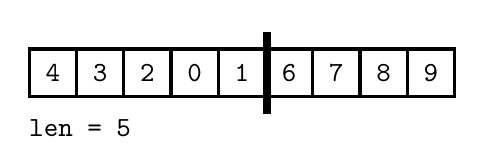
\begin{tikzpicture}

\draw (0.3, -0.3)
  node[draw, line width=0.04cm, , color=black,
       rounded corners=0cm, inner sep=0cm] {

\begin{minipage}[t][0.6cm]{0.6cm}
\mbox{}

\end{minipage}

};\draw (0.3, -0.3) node[color=black] {{\texttt{4}}};
\draw (0.8999999999999999, -0.3)
  node[draw, line width=0.04cm, , color=black,
       rounded corners=0cm, inner sep=0cm] {

\begin{minipage}[t][0.6cm]{0.6cm}
\mbox{}

\end{minipage}

};\draw (0.8999999999999999, -0.3) node[color=black] {{\texttt{3}}};
\draw (1.5, -0.3)
  node[draw, line width=0.04cm, , color=black,
       rounded corners=0cm, inner sep=0cm] {

\begin{minipage}[t][0.6cm]{0.6cm}
\mbox{}

\end{minipage}

};\draw (1.5, -0.3) node[color=black] {{\texttt{2}}};
\draw (2.0999999999999996, -0.3)
  node[draw, line width=0.04cm, , color=black,
       rounded corners=0cm, inner sep=0cm] {

\begin{minipage}[t][0.6cm]{0.6cm}
\mbox{}

\end{minipage}

};\draw (2.0999999999999996, -0.3) node[color=black] {{\texttt{0}}};
\draw (2.7, -0.3)
  node[draw, line width=0.04cm, , color=black,
       rounded corners=0cm, inner sep=0cm] {

\begin{minipage}[t][0.6cm]{0.6cm}
\mbox{}

\end{minipage}

};\draw (2.7, -0.3) node[color=black] {{\texttt{1}}};
\draw (3.3, -0.3)
  node[draw, line width=0.04cm, , color=black,
       rounded corners=0cm, inner sep=0cm] {

\begin{minipage}[t][0.6cm]{0.6cm}
\mbox{}

\end{minipage}

};\draw (3.3, -0.3) node[color=black] {{\texttt{6}}};
\draw (3.9, -0.3)
  node[draw, line width=0.04cm, , color=black,
       rounded corners=0cm, inner sep=0cm] {

\begin{minipage}[t][0.6cm]{0.6cm}
\mbox{}

\end{minipage}

};\draw (3.9, -0.3) node[color=black] {{\texttt{7}}};
\draw (4.5, -0.3)
  node[draw, line width=0.04cm, , color=black,
       rounded corners=0cm, inner sep=0cm] {

\begin{minipage}[t][0.6cm]{0.6cm}
\mbox{}

\end{minipage}

};\draw (4.5, -0.3) node[color=black] {{\texttt{8}}};
\draw (5.1, -0.3)
  node[draw, line width=0.04cm, , color=black,
       rounded corners=0cm, inner sep=0cm] {

\begin{minipage}[t][0.6cm]{0.6cm}
\mbox{}

\end{minipage}

};\draw (5.1, -0.3) node[color=black] {{\texttt{9}}};\draw[line width=0.1cm,black] (3.02,-0.82) to  (3.02,0.22);

\draw (1.0, -1.0)
  node[draw=none, line width=0cm, , color=black,
       rounded corners=0cm, inner sep=0cm] {

\begin{minipage}[t][0.1cm]{2cm}
\mbox{}

\end{minipage}

};
\draw (1.0, -1.0) node[color=black,
 inner sep=0cm] {
 
\begin{minipage}[t][0.1cm]{2cm}
\texttt{len = 5}
\end{minipage}

};
\end{tikzpicture}

\end{center}


the height at $\beta$ is also $h(T'_1)+2$.
This means that the whole tree must be balanced.



\underline{CASE LEFT-RIGHT: $k$ is inserted into the 
  right subtree of the left subtree of $\alpha$.}

\begin{center}

\begin{tikzpicture}
\node at (4,-0.8) [minimum size=8mm] (E) {$$};
\node at (3,-2.4000000000000004) [circle,draw,minimum size=8mm] (A) {$\alpha$};
\node at (1,-3.2) [circle,draw,minimum size=8mm] (C) {$\beta$};
\node at (5,-3.2)
    [isosceles triangle, shape border rotate=+90,
     draw,minimum size=8mm,
     anchor=north] (Btriangle) {$T'_3$};
\coordinate (B) at (5,-3.2);
\node at (0,-4.0)
    [isosceles triangle, shape border rotate=+90,
     draw,minimum size=8mm,
     anchor=north] (Dtriangle) {$T'_1$};
\coordinate (D) at (0,-4.0);
\node at (2,-4.0)
    [isosceles triangle, shape border rotate=+90,
     draw,minimum size=8mm,
     anchor=north] (Ftriangle) {$T'_2+k$};
\coordinate (F) at (2,-4.0);
\draw [-,thick] (A) -- (B);
\draw [-,thick] (A) -- (C);
\draw [-,thick] (E) -- (A);
\draw [-,thick] (C) -- (D);
\draw [-,thick] (C) -- (F);

;
\end{tikzpicture}
    
\end{center}


Let's look at $h(T'_1)$ and $h(T'_2)$.
Since $\beta$ is balanced, they are at most one away.
So $h(T'_2) = h(T'_1) + \ep$, $\ep = -1, 0, 1$.
If $\ep = -1$, then $T'_2$ is one shorter than
$T'_1$. In that case inserting $k$ into $T_2$
will mean that the height of $T_2$ will either
remain the same or increase by 1
which implies that the height at $\beta$
is unchanged.
This means that $\alpha$ cannot become unbalanced
after the insertion of $k$.
Also, $\ep$ cannot be 1 otherwise
after inserting $k$, $\beta$ becomes unbalanced
which contradicts the fact that the $\alpha$
is the lowest node to be unbalanced when $k$ is inserted.
Therefore $\ep$ must be $0$:
$h(T'_1) = h(T'_2)$.

Since adding $k$ to $T'_2$ unbalances $\alpha$, 
the lowest node of $T'_3$ must be 2 away from $k$ after it's inserted into 
$T'_2$.
Since $T'_2$ is one below $\beta$,
we must have $h(T'_2) = h(T'_3)$.

Therefore altogether $h(T'_1) = h(T'_2) = h(T'_3)$.

Look at this:

\begin{center}

\begin{tikzpicture}
\node at (3,-0.8) [minimum size=8mm] (E) {$$};
\node at (2,-2.4000000000000004) [circle,draw,minimum size=8mm] (C) {$\beta$};
\node at (0,-3.2)
    [isosceles triangle, shape border rotate=+90,
     draw,minimum size=8mm,
     anchor=north] (Dtriangle) {$T'_1$};
\coordinate (D) at (0,-3.2);
\node at (4,-3.2) [circle,draw,minimum size=8mm] (A) {$\alpha$};
\node at (2,-4.0)
    [isosceles triangle, shape border rotate=+90,
     draw,minimum size=8mm,
     anchor=north] (Ftriangle) {$T'_2+k$};
\coordinate (F) at (2,-4.0);
\node at (6,-4.0)
    [isosceles triangle, shape border rotate=+90,
     draw,minimum size=8mm,
     anchor=north] (Btriangle) {$T'_3$};
\coordinate (B) at (6,-4.0);
\draw [-,thick] (E) -- (C);
\draw [-,thick] (C) -- (D);
\draw [-,thick] (C) -- (A);
\draw [-,thick] (A) -- (F);
\draw [-,thick] (A) -- (B);

;
\end{tikzpicture}
    
\end{center}


This is NOT the right \lq\lq rotation".
(Find an example on your own to prove what I just said.)

The right thing to do is to do a \textit{left} rotation
at $\beta$ so that $\beta$ is \lq\lq heavier"
on the left and then then do a right rotation at $\alpha$.
Let me show you.
We start here where $k$ is now in $T''_2$ or $T''_3$:
\begin{center}
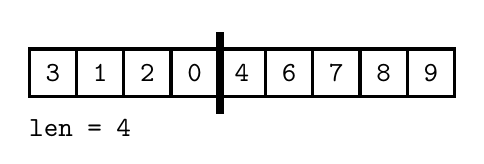
\begin{tikzpicture}

\draw (0.3, -0.3)
  node[draw, line width=0.04cm, , color=black,
       rounded corners=0cm, inner sep=0cm] {

\begin{minipage}[t][0.6cm]{0.6cm}
\mbox{}

\end{minipage}

};\draw (0.3, -0.3) node[color=black] {{\texttt{3}}};
\draw (0.8999999999999999, -0.3)
  node[draw, line width=0.04cm, , color=black,
       rounded corners=0cm, inner sep=0cm] {

\begin{minipage}[t][0.6cm]{0.6cm}
\mbox{}

\end{minipage}

};\draw (0.8999999999999999, -0.3) node[color=black] {{\texttt{1}}};
\draw (1.5, -0.3)
  node[draw, line width=0.04cm, , color=black,
       rounded corners=0cm, inner sep=0cm] {

\begin{minipage}[t][0.6cm]{0.6cm}
\mbox{}

\end{minipage}

};\draw (1.5, -0.3) node[color=black] {{\texttt{2}}};
\draw (2.0999999999999996, -0.3)
  node[draw, line width=0.04cm, , color=black,
       rounded corners=0cm, inner sep=0cm] {

\begin{minipage}[t][0.6cm]{0.6cm}
\mbox{}

\end{minipage}

};\draw (2.0999999999999996, -0.3) node[color=black] {{\texttt{0}}};
\draw (2.7, -0.3)
  node[draw, line width=0.04cm, , color=black,
       rounded corners=0cm, inner sep=0cm] {

\begin{minipage}[t][0.6cm]{0.6cm}
\mbox{}

\end{minipage}

};\draw (2.7, -0.3) node[color=black] {{\texttt{4}}};
\draw (3.3, -0.3)
  node[draw, line width=0.04cm, , color=black,
       rounded corners=0cm, inner sep=0cm] {

\begin{minipage}[t][0.6cm]{0.6cm}
\mbox{}

\end{minipage}

};\draw (3.3, -0.3) node[color=black] {{\texttt{6}}};
\draw (3.9, -0.3)
  node[draw, line width=0.04cm, , color=black,
       rounded corners=0cm, inner sep=0cm] {

\begin{minipage}[t][0.6cm]{0.6cm}
\mbox{}

\end{minipage}

};\draw (3.9, -0.3) node[color=black] {{\texttt{7}}};
\draw (4.5, -0.3)
  node[draw, line width=0.04cm, , color=black,
       rounded corners=0cm, inner sep=0cm] {

\begin{minipage}[t][0.6cm]{0.6cm}
\mbox{}

\end{minipage}

};\draw (4.5, -0.3) node[color=black] {{\texttt{8}}};
\draw (5.1, -0.3)
  node[draw, line width=0.04cm, , color=black,
       rounded corners=0cm, inner sep=0cm] {

\begin{minipage}[t][0.6cm]{0.6cm}
\mbox{}

\end{minipage}

};\draw (5.1, -0.3) node[color=black] {{\texttt{9}}};\draw[line width=0.1cm,black] (2.42,-0.82) to  (2.42,0.22);

\draw (1.0, -1.0)
  node[draw=none, line width=0cm, , color=black,
       rounded corners=0cm, inner sep=0cm] {

\begin{minipage}[t][0.1cm]{2cm}
\mbox{}

\end{minipage}

};
\draw (1.0, -1.0) node[color=black,
 inner sep=0cm] {
 
\begin{minipage}[t][0.1cm]{2cm}
\texttt{len = 4}
\end{minipage}

};
\end{tikzpicture}

\end{center}


After a left rotation at $\beta$, I get this:

\begin{center}

\begin{tikzpicture}
\node at (7,-0.8) [minimum size=8mm] (E) {$$};
\node at (5,-2.4000000000000004) [circle,draw,minimum size=8mm] (A) {$\alpha$};
\node at (3,-3.2) [circle,draw,minimum size=8mm] (F) {$\gamma$};
\node at (7,-3.2)
    [isosceles triangle, shape border rotate=+90,
     draw,minimum size=8mm,
     anchor=north] (Btriangle) {$T''_4$};
\coordinate (B) at (7,-3.2);
\node at (1,-4.0) [circle,draw,minimum size=8mm] (C) {$\beta$};
\node at (4,-4.0)
    [isosceles triangle, shape border rotate=+90,
     draw,minimum size=8mm,
     anchor=north] (Htriangle) {$T''_3$};
\coordinate (H) at (4,-4.0);
\node at (0,-4.800000000000001)
    [isosceles triangle, shape border rotate=+90,
     draw,minimum size=8mm,
     anchor=north] (Dtriangle) {$T''_1$};
\coordinate (D) at (0,-4.800000000000001);
\node at (2,-4.800000000000001)
    [isosceles triangle, shape border rotate=+90,
     draw,minimum size=8mm,
     anchor=north] (Gtriangle) {$T''_2$};
\coordinate (G) at (2,-4.800000000000001);
\draw [-,thick] (E) -- (A);
\draw [-,thick] (A) -- (F);
\draw [-,thick] (A) -- (B);
\draw [-,thick] (F) -- (C);
\draw [-,thick] (F) -- (H);
\draw [-,thick] (C) -- (D);
\draw [-,thick] (C) -- (G);
\draw [-,thick] (A) -- (B);

;
\end{tikzpicture}
    
\end{center}


Now I right rotation at $\alpha$ to get this:
\begin{center}
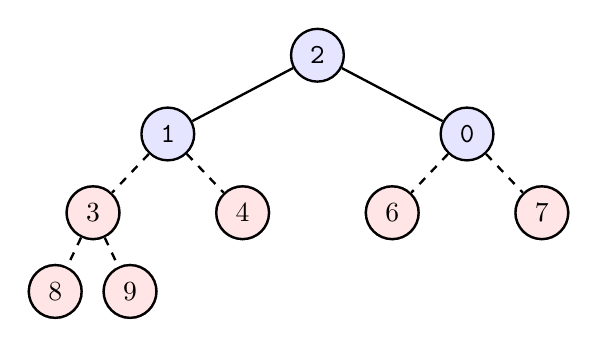
\begin{tikzpicture}

\fill[blue!10] (0.0, 0.0) circle (0.35);
\node [line width=0.03cm,black,minimum size=0.6699999999999999cm,draw,circle] at (0.0,0.0)(2){};\draw (0.0, 0.0) node[color=black] {\texttt{2}};
\fill[blue!10] (-1.9, -1.0) circle (0.35);
\node [line width=0.03cm,black,minimum size=0.6699999999999999cm,draw,circle] at (-1.9,-1.0)(1){};\draw (-1.9, -1.0) node[color=black] {\texttt{1}};
\fill[blue!10] (1.9, -1.0) circle (0.35);
\node [line width=0.03cm,black,minimum size=0.6699999999999999cm,draw,circle] at (1.9,-1.0)(0){};\draw (1.9, -1.0) node[color=black] {\texttt{0}};
\fill[blue!10] (-2.85, -2.0) circle (0.35);
\node [line width=0.03cm,black,minimum size=0.6699999999999999cm,draw,circle] at (-2.85,-2.0)(3){};\draw (-2.85, -2.0) node[color=black] {\texttt{3}};
\fill[blue!10] (-0.95, -2.0) circle (0.35);
\node [line width=0.03cm,black,minimum size=0.6699999999999999cm,draw,circle] at (-0.95,-2.0)(4){};\draw (-0.95, -2.0) node[color=black] {\texttt{4}};
\fill[blue!10] (0.95, -2.0) circle (0.35);
\node [line width=0.03cm,black,minimum size=0.6699999999999999cm,draw,circle] at (0.95,-2.0)(6){};\draw (0.95, -2.0) node[color=black] {\texttt{6}};
\fill[blue!10] (2.85, -2.0) circle (0.35);
\node [line width=0.03cm,black,minimum size=0.6699999999999999cm,draw,circle] at (2.85,-2.0)(7){};\draw (2.85, -2.0) node[color=black] {\texttt{7}};
\fill[blue!10] (-3.33, -3.0) circle (0.35);
\node [line width=0.03cm,black,minimum size=0.6699999999999999cm,draw,circle] at (-3.33,-3.0)(8){};\draw (-3.33, -3.0) node[color=black] {\texttt{8}};
\fill[blue!10] (-2.38, -3.0) circle (0.35);
\node [line width=0.03cm,black,minimum size=0.6699999999999999cm,draw,circle] at (-2.38,-3.0)(9){};\draw (-2.38, -3.0) node[color=black] {\texttt{9}};\draw[line width=0.03cm,black] (2) to  (1);
\draw[line width=0.03cm,black] (2) to  (0);
\draw[line width=0.03cm,black] (1) to  (3);
\draw[line width=0.03cm,black] (1) to  (4);
\draw[line width=0.03cm,black] (0) to  (6);
\draw[line width=0.03cm,black] (0) to  (7);
\draw[line width=0.03cm,black] (3) to  (8);
\draw[line width=0.03cm,black] (3) to  (9);

\fill[red!10] (-2.38, -3.0) circle (0.35);
\draw[line width=0.03cm,black] (-2.38, -3.0) circle (0.33499999999999996);\draw (-2.38, -3.0) node[color=black] {9};
\fill[red!10] (-3.33, -3.0) circle (0.35);
\draw[line width=0.03cm,black] (-3.33, -3.0) circle (0.33499999999999996);\draw (-3.33, -3.0) node[color=black] {8};
\fill[red!10] (2.85, -2.0) circle (0.35);
\draw[line width=0.03cm,black] (2.85, -2.0) circle (0.33499999999999996);\draw (2.85, -2.0) node[color=black] {7};
\fill[red!10] (0.95, -2.0) circle (0.35);
\draw[line width=0.03cm,black] (0.95, -2.0) circle (0.33499999999999996);\draw (0.95, -2.0) node[color=black] {6};
\fill[red!10] (-0.95, -2.0) circle (0.35);
\draw[line width=0.03cm,black] (-0.95, -2.0) circle (0.33499999999999996);\draw (-0.95, -2.0) node[color=black] {4};
\fill[red!10] (-2.85, -2.0) circle (0.35);
\draw[line width=0.03cm,black] (-2.85, -2.0) circle (0.33499999999999996);\draw (-2.85, -2.0) node[color=black] {3};\draw[line width=0.1cm,white] (3) to  (9);
\draw[line width=0.03cm,black,,dashed] (3) to  (9);
\draw[line width=0.1cm,white] (3) to  (8);
\draw[line width=0.03cm,black,,dashed] (3) to  (8);
\draw[line width=0.1cm,white] (0) to  (7);
\draw[line width=0.03cm,black,,dashed] (0) to  (7);
\draw[line width=0.1cm,white] (0) to  (6);
\draw[line width=0.03cm,black,,dashed] (0) to  (6);
\draw[line width=0.1cm,white] (1) to  (4);
\draw[line width=0.03cm,black,,dashed] (1) to  (4);
\draw[line width=0.1cm,white] (1) to  (3);
\draw[line width=0.03cm,black,,dashed] (1) to  (3);
\end{tikzpicture}

\end{center}



Let me summarize.
Suppose after inserting a node $k$ into a BST,
$\alpha$ is the lower node that is unbalanced.
\begin{tightlist}
\li LEFT-LEFT CASE: If $k$ took a left-left direction from $\alpha$,
then you should do a right rotation.
\li LEFT-RIGHT: If $k$ took at left-right direction from $\alpha$,
then you should a left rotation on the left child $\beta$ of $\alpha$
followed by a right rotation at $\beta$ which occupies the original 
position of $\alpha$.
\end{tightlist}

If should not be too surprising that the mirror image of
the above is true:
Suppose after inserting a node $k$ into a BST,
$\alpha$ is the lower node that is unbalanced.
\begin{tightlist}
\li RIGHT-RIGHT CASE: If $k$ took a right-right direction from $\alpha$,
then you should do a left rotation.
\li RIGHT-LEFT: If $k$ took at right-left direction from $\alpha$,
then you should a right rotation on the right child $\beta$ of $\alpha$
followed by a left rotation at $\beta$ which occupies the original 
position of $\alpha$.
\end{tightlist}
Draw a picture similar to the above to see what's happening.

\newpage
\subsection{AVL trees}

An AVL tree $T$ is a tree that is self-balancing BST in the sense that
the insert and delete operations include self-balancing operations
(using left and right rotations) so that the tree is balanced after each
insert or delete operation.

\newpage
\subsection{AVL insert}
Suppose a node $n$ is inserted into $T$.
Suppose the new tree is $T'$.
There's a path from the root of $T'$ to $n$.
You go up along this path and when you are at a node $m$
that is unbalanced (i.e., the subtree with $m$ as root
is unbalanced), we balance at $m$:
\begin{tightlist}
  \li CASE: left-left. If the path from $m$ along $P$ going down to the new node is
  left-left,
  you perform a right rotation at $m$.
  \li CASE: left-right. If the path from $m$ along $P$ going down to the new node is
  left-right,
  you perform a left rotation one step below $m$ and then a right rotation at $m$.
  \li CASE: right-right. If the path from $m$ along $P$ going down to the new node is
  right-right,
  you perform a left rotation at $m$.
  \li CASE: right-left. If the path from $m$ along $P$ going down to the new node is
  right-left,
  you perform a right rotation one step below $m$ and then a left rotation at $m$.
\end{tightlist}

For instance suppose I start off with this:

\begin{center}
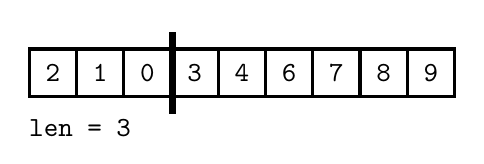
\begin{tikzpicture}

\draw (0.3, -0.3)
  node[draw, line width=0.04cm, , color=black,
       rounded corners=0cm, inner sep=0cm] {

\begin{minipage}[t][0.6cm]{0.6cm}
\mbox{}

\end{minipage}

};\draw (0.3, -0.3) node[color=black] {{\texttt{2}}};
\draw (0.8999999999999999, -0.3)
  node[draw, line width=0.04cm, , color=black,
       rounded corners=0cm, inner sep=0cm] {

\begin{minipage}[t][0.6cm]{0.6cm}
\mbox{}

\end{minipage}

};\draw (0.8999999999999999, -0.3) node[color=black] {{\texttt{1}}};
\draw (1.5, -0.3)
  node[draw, line width=0.04cm, , color=black,
       rounded corners=0cm, inner sep=0cm] {

\begin{minipage}[t][0.6cm]{0.6cm}
\mbox{}

\end{minipage}

};\draw (1.5, -0.3) node[color=black] {{\texttt{0}}};
\draw (2.0999999999999996, -0.3)
  node[draw, line width=0.04cm, , color=black,
       rounded corners=0cm, inner sep=0cm] {

\begin{minipage}[t][0.6cm]{0.6cm}
\mbox{}

\end{minipage}

};\draw (2.0999999999999996, -0.3) node[color=black] {{\texttt{3}}};
\draw (2.7, -0.3)
  node[draw, line width=0.04cm, , color=black,
       rounded corners=0cm, inner sep=0cm] {

\begin{minipage}[t][0.6cm]{0.6cm}
\mbox{}

\end{minipage}

};\draw (2.7, -0.3) node[color=black] {{\texttt{4}}};
\draw (3.3, -0.3)
  node[draw, line width=0.04cm, , color=black,
       rounded corners=0cm, inner sep=0cm] {

\begin{minipage}[t][0.6cm]{0.6cm}
\mbox{}

\end{minipage}

};\draw (3.3, -0.3) node[color=black] {{\texttt{6}}};
\draw (3.9, -0.3)
  node[draw, line width=0.04cm, , color=black,
       rounded corners=0cm, inner sep=0cm] {

\begin{minipage}[t][0.6cm]{0.6cm}
\mbox{}

\end{minipage}

};\draw (3.9, -0.3) node[color=black] {{\texttt{7}}};
\draw (4.5, -0.3)
  node[draw, line width=0.04cm, , color=black,
       rounded corners=0cm, inner sep=0cm] {

\begin{minipage}[t][0.6cm]{0.6cm}
\mbox{}

\end{minipage}

};\draw (4.5, -0.3) node[color=black] {{\texttt{8}}};
\draw (5.1, -0.3)
  node[draw, line width=0.04cm, , color=black,
       rounded corners=0cm, inner sep=0cm] {

\begin{minipage}[t][0.6cm]{0.6cm}
\mbox{}

\end{minipage}

};\draw (5.1, -0.3) node[color=black] {{\texttt{9}}};\draw[line width=0.1cm,black] (1.82,-0.82) to  (1.82,0.22);

\draw (1.0, -1.0)
  node[draw=none, line width=0cm, , color=black,
       rounded corners=0cm, inner sep=0cm] {

\begin{minipage}[t][0.1cm]{2cm}
\mbox{}

\end{minipage}

};
\draw (1.0, -1.0) node[color=black,
 inner sep=0cm] {
 
\begin{minipage}[t][0.1cm]{2cm}
\texttt{len = 3}
\end{minipage}

};
\end{tikzpicture}

\end{center}



This is height balanced.
After I insert 2, I get:

\begin{center}
\begin{tikzpicture}

\fill[white] (0.0, 0.0) circle (0.3);
\node [line width=0.03cm,black,minimum size=0.57cm,draw,circle] at (0.0,0.0)(10){};\draw (0.0, 0.0) node[color=black] {\texttt{10}};
\fill[white] (-1.5, -1.0) circle (0.3);
\node [line width=0.03cm,black,minimum size=0.57cm,draw,circle] at (-1.5,-1.0)(5){};\draw (-1.5, -1.0) node[color=black] {\texttt{5}};
\fill[white] (1.5, -1.0) circle (0.3);
\node [line width=0.03cm,black,minimum size=0.57cm,draw,circle] at (1.5,-1.0)(18){};\draw (1.5, -1.0) node[color=black] {\texttt{18}};
\fill[white] (-2.25, -2.0) circle (0.3);
\node [line width=0.03cm,black,minimum size=0.57cm,draw,circle] at (-2.25,-2.0)(2){};\draw (-2.25, -2.0) node[color=black] {\texttt{2}};\draw[line width=0.03cm,black,->,>=triangle 60] (10) to  (5);
\draw[line width=0.03cm,black,->,>=triangle 60] (10) to  (18);
\draw[line width=0.03cm,black,->,>=triangle 60] (5) to  (2);
\end{tikzpicture}

\end{center}



Checking all the nodes along the insertion path,
I see that they are all balanced.
(Make sure you check that.)
Now if I insert a 0, I get this:

\begin{center}
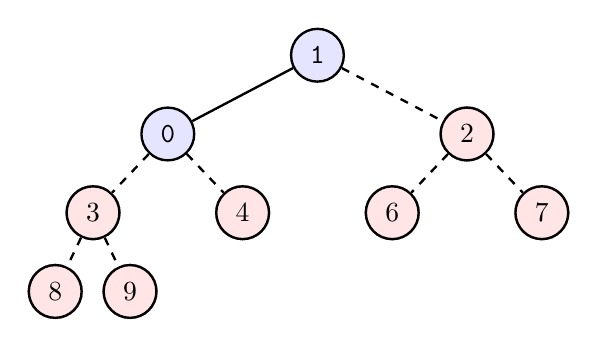
\begin{tikzpicture}

\fill[blue!10] (0.0, 0.0) circle (0.35);
\node [line width=0.03cm,black,minimum size=0.6699999999999999cm,draw,circle] at (0.0,0.0)(1){};\draw (0.0, 0.0) node[color=black] {\texttt{1}};
\fill[blue!10] (-1.9, -1.0) circle (0.35);
\node [line width=0.03cm,black,minimum size=0.6699999999999999cm,draw,circle] at (-1.9,-1.0)(0){};\draw (-1.9, -1.0) node[color=black] {\texttt{0}};
\fill[blue!10] (1.9, -1.0) circle (0.35);
\node [line width=0.03cm,black,minimum size=0.6699999999999999cm,draw,circle] at (1.9,-1.0)(2){};\draw (1.9, -1.0) node[color=black] {\texttt{2}};
\fill[blue!10] (-2.85, -2.0) circle (0.35);
\node [line width=0.03cm,black,minimum size=0.6699999999999999cm,draw,circle] at (-2.85,-2.0)(3){};\draw (-2.85, -2.0) node[color=black] {\texttt{3}};
\fill[blue!10] (-0.95, -2.0) circle (0.35);
\node [line width=0.03cm,black,minimum size=0.6699999999999999cm,draw,circle] at (-0.95,-2.0)(4){};\draw (-0.95, -2.0) node[color=black] {\texttt{4}};
\fill[blue!10] (0.95, -2.0) circle (0.35);
\node [line width=0.03cm,black,minimum size=0.6699999999999999cm,draw,circle] at (0.95,-2.0)(6){};\draw (0.95, -2.0) node[color=black] {\texttt{6}};
\fill[blue!10] (2.85, -2.0) circle (0.35);
\node [line width=0.03cm,black,minimum size=0.6699999999999999cm,draw,circle] at (2.85,-2.0)(7){};\draw (2.85, -2.0) node[color=black] {\texttt{7}};
\fill[blue!10] (-3.33, -3.0) circle (0.35);
\node [line width=0.03cm,black,minimum size=0.6699999999999999cm,draw,circle] at (-3.33,-3.0)(8){};\draw (-3.33, -3.0) node[color=black] {\texttt{8}};
\fill[blue!10] (-2.38, -3.0) circle (0.35);
\node [line width=0.03cm,black,minimum size=0.6699999999999999cm,draw,circle] at (-2.38,-3.0)(9){};\draw (-2.38, -3.0) node[color=black] {\texttt{9}};\draw[line width=0.03cm,black] (1) to  (0);
\draw[line width=0.03cm,black] (1) to  (2);
\draw[line width=0.03cm,black] (0) to  (3);
\draw[line width=0.03cm,black] (0) to  (4);
\draw[line width=0.03cm,black] (2) to  (6);
\draw[line width=0.03cm,black] (2) to  (7);
\draw[line width=0.03cm,black] (3) to  (8);
\draw[line width=0.03cm,black] (3) to  (9);

\fill[red!10] (-2.38, -3.0) circle (0.35);
\draw[line width=0.03cm,black] (-2.38, -3.0) circle (0.33499999999999996);\draw (-2.38, -3.0) node[color=black] {9};
\fill[red!10] (-3.33, -3.0) circle (0.35);
\draw[line width=0.03cm,black] (-3.33, -3.0) circle (0.33499999999999996);\draw (-3.33, -3.0) node[color=black] {8};
\fill[red!10] (2.85, -2.0) circle (0.35);
\draw[line width=0.03cm,black] (2.85, -2.0) circle (0.33499999999999996);\draw (2.85, -2.0) node[color=black] {7};
\fill[red!10] (0.95, -2.0) circle (0.35);
\draw[line width=0.03cm,black] (0.95, -2.0) circle (0.33499999999999996);\draw (0.95, -2.0) node[color=black] {6};
\fill[red!10] (-0.95, -2.0) circle (0.35);
\draw[line width=0.03cm,black] (-0.95, -2.0) circle (0.33499999999999996);\draw (-0.95, -2.0) node[color=black] {4};
\fill[red!10] (-2.85, -2.0) circle (0.35);
\draw[line width=0.03cm,black] (-2.85, -2.0) circle (0.33499999999999996);\draw (-2.85, -2.0) node[color=black] {3};
\fill[red!10] (1.9, -1.0) circle (0.35);
\draw[line width=0.03cm,black] (1.9, -1.0) circle (0.33499999999999996);\draw (1.9, -1.0) node[color=black] {2};\draw[line width=0.1cm,white] (1) to  (2);
\draw[line width=0.03cm,black,,dashed] (1) to  (2);
\draw[line width=0.1cm,white] (3) to  (9);
\draw[line width=0.03cm,black,,dashed] (3) to  (9);
\draw[line width=0.1cm,white] (3) to  (8);
\draw[line width=0.03cm,black,,dashed] (3) to  (8);
\draw[line width=0.1cm,white] (2) to  (7);
\draw[line width=0.03cm,black,,dashed] (2) to  (7);
\draw[line width=0.1cm,white] (2) to  (6);
\draw[line width=0.03cm,black,,dashed] (2) to  (6);
\draw[line width=0.1cm,white] (0) to  (4);
\draw[line width=0.03cm,black,,dashed] (0) to  (4);
\draw[line width=0.1cm,white] (0) to  (3);
\draw[line width=0.03cm,black,,dashed] (0) to  (3);
\end{tikzpicture}

\end{center}



The path of insertion is in red.

When I go back up the tree from the new node, I see that
the first node that is not balanced is 5:

\begin{center}
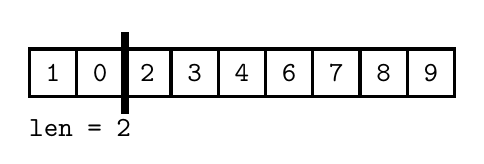
\begin{tikzpicture}

\draw (0.3, -0.3)
  node[draw, line width=0.04cm, , color=black,
       rounded corners=0cm, inner sep=0cm] {

\begin{minipage}[t][0.6cm]{0.6cm}
\mbox{}

\end{minipage}

};\draw (0.3, -0.3) node[color=black] {{\texttt{1}}};
\draw (0.8999999999999999, -0.3)
  node[draw, line width=0.04cm, , color=black,
       rounded corners=0cm, inner sep=0cm] {

\begin{minipage}[t][0.6cm]{0.6cm}
\mbox{}

\end{minipage}

};\draw (0.8999999999999999, -0.3) node[color=black] {{\texttt{0}}};
\draw (1.5, -0.3)
  node[draw, line width=0.04cm, , color=black,
       rounded corners=0cm, inner sep=0cm] {

\begin{minipage}[t][0.6cm]{0.6cm}
\mbox{}

\end{minipage}

};\draw (1.5, -0.3) node[color=black] {{\texttt{2}}};
\draw (2.0999999999999996, -0.3)
  node[draw, line width=0.04cm, , color=black,
       rounded corners=0cm, inner sep=0cm] {

\begin{minipage}[t][0.6cm]{0.6cm}
\mbox{}

\end{minipage}

};\draw (2.0999999999999996, -0.3) node[color=black] {{\texttt{3}}};
\draw (2.7, -0.3)
  node[draw, line width=0.04cm, , color=black,
       rounded corners=0cm, inner sep=0cm] {

\begin{minipage}[t][0.6cm]{0.6cm}
\mbox{}

\end{minipage}

};\draw (2.7, -0.3) node[color=black] {{\texttt{4}}};
\draw (3.3, -0.3)
  node[draw, line width=0.04cm, , color=black,
       rounded corners=0cm, inner sep=0cm] {

\begin{minipage}[t][0.6cm]{0.6cm}
\mbox{}

\end{minipage}

};\draw (3.3, -0.3) node[color=black] {{\texttt{6}}};
\draw (3.9, -0.3)
  node[draw, line width=0.04cm, , color=black,
       rounded corners=0cm, inner sep=0cm] {

\begin{minipage}[t][0.6cm]{0.6cm}
\mbox{}

\end{minipage}

};\draw (3.9, -0.3) node[color=black] {{\texttt{7}}};
\draw (4.5, -0.3)
  node[draw, line width=0.04cm, , color=black,
       rounded corners=0cm, inner sep=0cm] {

\begin{minipage}[t][0.6cm]{0.6cm}
\mbox{}

\end{minipage}

};\draw (4.5, -0.3) node[color=black] {{\texttt{8}}};
\draw (5.1, -0.3)
  node[draw, line width=0.04cm, , color=black,
       rounded corners=0cm, inner sep=0cm] {

\begin{minipage}[t][0.6cm]{0.6cm}
\mbox{}

\end{minipage}

};\draw (5.1, -0.3) node[color=black] {{\texttt{9}}};\draw[line width=0.1cm,black] (1.22,-0.82) to  (1.22,0.22);

\draw (1.0, -1.0)
  node[draw=none, line width=0cm, , color=black,
       rounded corners=0cm, inner sep=0cm] {

\begin{minipage}[t][0.1cm]{2cm}
\mbox{}

\end{minipage}

};
\draw (1.0, -1.0) node[color=black,
 inner sep=0cm] {
 
\begin{minipage}[t][0.1cm]{2cm}
\texttt{len = 2}
\end{minipage}

};
\end{tikzpicture}

\end{center}



Along this path, at 5, I took two lefts down -- we are in the left-left case.
Therefore I will perform a right rotation at 5 to get:

\begin{center}
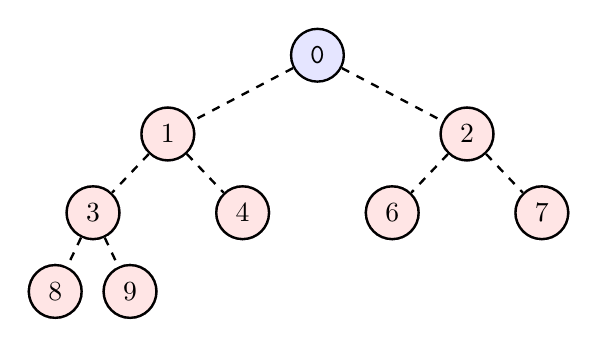
\begin{tikzpicture}

\fill[blue!10] (0.0, 0.0) circle (0.35);
\node [line width=0.03cm,black,minimum size=0.6699999999999999cm,draw,circle] at (0.0,0.0)(0){};\draw (0.0, 0.0) node[color=black] {\texttt{0}};
\fill[blue!10] (-1.9, -1.0) circle (0.35);
\node [line width=0.03cm,black,minimum size=0.6699999999999999cm,draw,circle] at (-1.9,-1.0)(1){};\draw (-1.9, -1.0) node[color=black] {\texttt{1}};
\fill[blue!10] (1.9, -1.0) circle (0.35);
\node [line width=0.03cm,black,minimum size=0.6699999999999999cm,draw,circle] at (1.9,-1.0)(2){};\draw (1.9, -1.0) node[color=black] {\texttt{2}};
\fill[blue!10] (-2.85, -2.0) circle (0.35);
\node [line width=0.03cm,black,minimum size=0.6699999999999999cm,draw,circle] at (-2.85,-2.0)(3){};\draw (-2.85, -2.0) node[color=black] {\texttt{3}};
\fill[blue!10] (-0.95, -2.0) circle (0.35);
\node [line width=0.03cm,black,minimum size=0.6699999999999999cm,draw,circle] at (-0.95,-2.0)(4){};\draw (-0.95, -2.0) node[color=black] {\texttt{4}};
\fill[blue!10] (0.95, -2.0) circle (0.35);
\node [line width=0.03cm,black,minimum size=0.6699999999999999cm,draw,circle] at (0.95,-2.0)(6){};\draw (0.95, -2.0) node[color=black] {\texttt{6}};
\fill[blue!10] (2.85, -2.0) circle (0.35);
\node [line width=0.03cm,black,minimum size=0.6699999999999999cm,draw,circle] at (2.85,-2.0)(7){};\draw (2.85, -2.0) node[color=black] {\texttt{7}};
\fill[blue!10] (-3.33, -3.0) circle (0.35);
\node [line width=0.03cm,black,minimum size=0.6699999999999999cm,draw,circle] at (-3.33,-3.0)(8){};\draw (-3.33, -3.0) node[color=black] {\texttt{8}};
\fill[blue!10] (-2.38, -3.0) circle (0.35);
\node [line width=0.03cm,black,minimum size=0.6699999999999999cm,draw,circle] at (-2.38,-3.0)(9){};\draw (-2.38, -3.0) node[color=black] {\texttt{9}};\draw[line width=0.03cm,black] (0) to  (1);
\draw[line width=0.03cm,black] (0) to  (2);
\draw[line width=0.03cm,black] (1) to  (3);
\draw[line width=0.03cm,black] (1) to  (4);
\draw[line width=0.03cm,black] (2) to  (6);
\draw[line width=0.03cm,black] (2) to  (7);
\draw[line width=0.03cm,black] (3) to  (8);
\draw[line width=0.03cm,black] (3) to  (9);

\fill[red!10] (-2.38, -3.0) circle (0.35);
\draw[line width=0.03cm,black] (-2.38, -3.0) circle (0.33499999999999996);\draw (-2.38, -3.0) node[color=black] {9};
\fill[red!10] (-3.33, -3.0) circle (0.35);
\draw[line width=0.03cm,black] (-3.33, -3.0) circle (0.33499999999999996);\draw (-3.33, -3.0) node[color=black] {8};
\fill[red!10] (2.85, -2.0) circle (0.35);
\draw[line width=0.03cm,black] (2.85, -2.0) circle (0.33499999999999996);\draw (2.85, -2.0) node[color=black] {7};
\fill[red!10] (0.95, -2.0) circle (0.35);
\draw[line width=0.03cm,black] (0.95, -2.0) circle (0.33499999999999996);\draw (0.95, -2.0) node[color=black] {6};
\fill[red!10] (-0.95, -2.0) circle (0.35);
\draw[line width=0.03cm,black] (-0.95, -2.0) circle (0.33499999999999996);\draw (-0.95, -2.0) node[color=black] {4};
\fill[red!10] (-2.85, -2.0) circle (0.35);
\draw[line width=0.03cm,black] (-2.85, -2.0) circle (0.33499999999999996);\draw (-2.85, -2.0) node[color=black] {3};
\fill[red!10] (1.9, -1.0) circle (0.35);
\draw[line width=0.03cm,black] (1.9, -1.0) circle (0.33499999999999996);\draw (1.9, -1.0) node[color=black] {2};
\fill[red!10] (-1.9, -1.0) circle (0.35);
\draw[line width=0.03cm,black] (-1.9, -1.0) circle (0.33499999999999996);\draw (-1.9, -1.0) node[color=black] {1};\draw[line width=0.1cm,white] (3) to  (9);
\draw[line width=0.03cm,black,,dashed] (3) to  (9);
\draw[line width=0.1cm,white] (3) to  (8);
\draw[line width=0.03cm,black,,dashed] (3) to  (8);
\draw[line width=0.1cm,white] (2) to  (7);
\draw[line width=0.03cm,black,,dashed] (2) to  (7);
\draw[line width=0.1cm,white] (2) to  (6);
\draw[line width=0.03cm,black,,dashed] (2) to  (6);
\draw[line width=0.1cm,white] (1) to  (4);
\draw[line width=0.03cm,black,,dashed] (1) to  (4);
\draw[line width=0.1cm,white] (1) to  (3);
\draw[line width=0.03cm,black,,dashed] (1) to  (3);
\draw[line width=0.1cm,white] (0) to  (1);
\draw[line width=0.03cm,black,,dashed] (0) to  (1);
\draw[line width=0.1cm,white] (0) to  (2);
\draw[line width=0.03cm,black,,dashed] (0) to  (2);
\end{tikzpicture}

\end{center}



The tree is now balanced at 2 (the previous location of 5).
it's also balanced at 10.

If I insert a 3, I get this:

\begin{center}
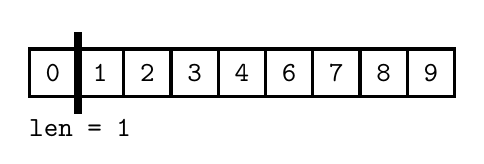
\begin{tikzpicture}

\draw (0.3, -0.3)
  node[draw, line width=0.04cm, , color=black,
       rounded corners=0cm, inner sep=0cm] {

\begin{minipage}[t][0.6cm]{0.6cm}
\mbox{}

\end{minipage}

};\draw (0.3, -0.3) node[color=black] {{\texttt{0}}};
\draw (0.8999999999999999, -0.3)
  node[draw, line width=0.04cm, , color=black,
       rounded corners=0cm, inner sep=0cm] {

\begin{minipage}[t][0.6cm]{0.6cm}
\mbox{}

\end{minipage}

};\draw (0.8999999999999999, -0.3) node[color=black] {{\texttt{1}}};
\draw (1.5, -0.3)
  node[draw, line width=0.04cm, , color=black,
       rounded corners=0cm, inner sep=0cm] {

\begin{minipage}[t][0.6cm]{0.6cm}
\mbox{}

\end{minipage}

};\draw (1.5, -0.3) node[color=black] {{\texttt{2}}};
\draw (2.0999999999999996, -0.3)
  node[draw, line width=0.04cm, , color=black,
       rounded corners=0cm, inner sep=0cm] {

\begin{minipage}[t][0.6cm]{0.6cm}
\mbox{}

\end{minipage}

};\draw (2.0999999999999996, -0.3) node[color=black] {{\texttt{3}}};
\draw (2.7, -0.3)
  node[draw, line width=0.04cm, , color=black,
       rounded corners=0cm, inner sep=0cm] {

\begin{minipage}[t][0.6cm]{0.6cm}
\mbox{}

\end{minipage}

};\draw (2.7, -0.3) node[color=black] {{\texttt{4}}};
\draw (3.3, -0.3)
  node[draw, line width=0.04cm, , color=black,
       rounded corners=0cm, inner sep=0cm] {

\begin{minipage}[t][0.6cm]{0.6cm}
\mbox{}

\end{minipage}

};\draw (3.3, -0.3) node[color=black] {{\texttt{6}}};
\draw (3.9, -0.3)
  node[draw, line width=0.04cm, , color=black,
       rounded corners=0cm, inner sep=0cm] {

\begin{minipage}[t][0.6cm]{0.6cm}
\mbox{}

\end{minipage}

};\draw (3.9, -0.3) node[color=black] {{\texttt{7}}};
\draw (4.5, -0.3)
  node[draw, line width=0.04cm, , color=black,
       rounded corners=0cm, inner sep=0cm] {

\begin{minipage}[t][0.6cm]{0.6cm}
\mbox{}

\end{minipage}

};\draw (4.5, -0.3) node[color=black] {{\texttt{8}}};
\draw (5.1, -0.3)
  node[draw, line width=0.04cm, , color=black,
       rounded corners=0cm, inner sep=0cm] {

\begin{minipage}[t][0.6cm]{0.6cm}
\mbox{}

\end{minipage}

};\draw (5.1, -0.3) node[color=black] {{\texttt{9}}};\draw[line width=0.1cm,black] (0.62,-0.82) to  (0.62,0.22);

\draw (1.0, -1.0)
  node[draw=none, line width=0cm, , color=black,
       rounded corners=0cm, inner sep=0cm] {

\begin{minipage}[t][0.1cm]{2cm}
\mbox{}

\end{minipage}

};
\draw (1.0, -1.0) node[color=black,
 inner sep=0cm] {
 
\begin{minipage}[t][0.1cm]{2cm}
\texttt{len = 1}
\end{minipage}

};
\end{tikzpicture}

\end{center}



The part of insertion is shown in red.
Going up along the path of insertion, the first node that is unbalanced
is 10.
At 10, going down, I take a left (at 10) then a right (at 2).
Therefore, I will first make a left rotation at 2, and then a right rotation at 10.
The left rotation at 2 gives me this:


\begin{center}

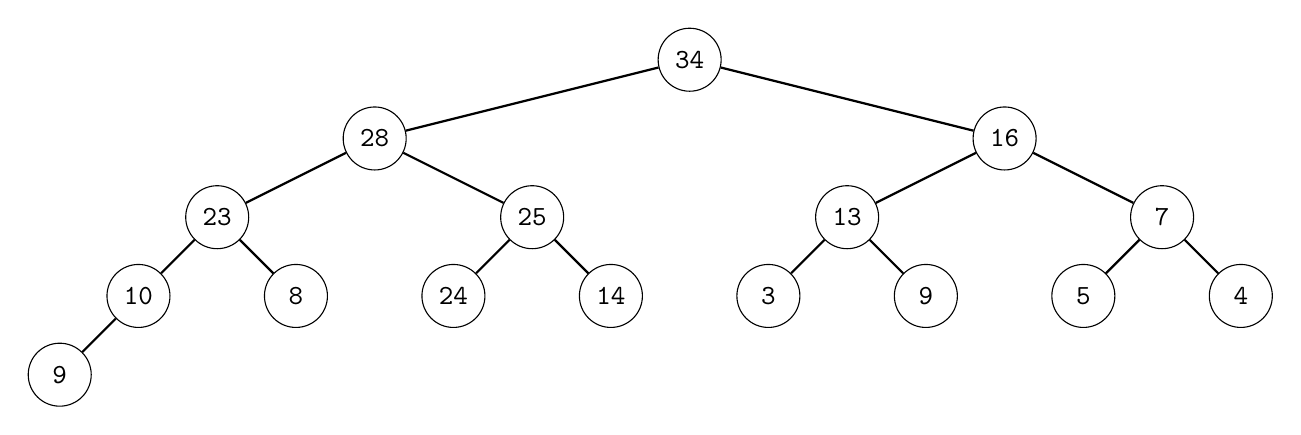
\begin{tikzpicture}
\node at (8,-1) [circle,draw,minimum size=8mm] (A) {\texttt{34}};
\node at (4,-2) [circle,draw,minimum size=8mm] (B) {\texttt{28}};
\node at (12,-2) [circle,draw,minimum size=8mm] (C) {\texttt{16}};
\node at (2,-3) [circle,draw,minimum size=8mm] (D) {\texttt{23}};
\node at (6,-3) [circle,draw,minimum size=8mm] (E) {\texttt{25}};
\node at (10,-3) [circle,draw,minimum size=8mm] (F) {\texttt{13}};
\node at (14,-3) [circle,draw,minimum size=8mm] (G) {\texttt{7}};
\node at (1,-4) [circle,draw,minimum size=8mm] (H) {\texttt{10}};
\node at (3,-4) [circle,draw,minimum size=8mm] (I) {\texttt{8}};
\node at (5,-4) [circle,draw,minimum size=8mm] (J) {\texttt{24}};
\node at (7,-4) [circle,draw,minimum size=8mm] (K) {\texttt{14}};
\node at (9,-4) [circle,draw,minimum size=8mm] (L) {\texttt{3}};
\node at (11,-4) [circle,draw,minimum size=8mm] (M) {\texttt{9}};
\node at (13,-4) [circle,draw,minimum size=8mm] (N) {\texttt{5}};
\node at (15,-4) [circle,draw,minimum size=8mm] (O) {\texttt{4}};
\node at (0,-5) [circle,draw,minimum size=8mm] (P) {\texttt{9}};
\draw [-,thick] (A) -- (B);
\draw [-,thick] (A) -- (C);
\draw [-,thick] (B) -- (D);
\draw [-,thick] (B) -- (E);
\draw [-,thick] (C) -- (G);
\draw [-,thick] (C) -- (F);
\draw [-,thick] (D) -- (H);
\draw [-,thick] (D) -- (I);
\draw [-,thick] (E) -- (J);
\draw [-,thick] (E) -- (K);
\draw [-,thick] (F) -- (L);
\draw [-,thick] (F) -- (M);
\draw [-,thick] (G) -- (N);
\draw [-,thick] (G) -- (O);
\draw [-,thick] (H) -- (P);

;
\end{tikzpicture}
    
\end{center}



and then I do a right rotation at 10:

\begin{center}
\begin{tikzpicture}

\fill[white] (0.0, 0.0) circle (0.3);
\node [line width=0.03cm,black,minimum size=0.57cm,draw,circle] at (0.0,0.0)(5){};\draw (0.0, 0.0) node[color=black] {\texttt{5}};
\fill[white] (-1.5, -1.0) circle (0.3);
\node [line width=0.03cm,black,minimum size=0.57cm,draw,circle] at (-1.5,-1.0)(2){};\draw (-1.5, -1.0) node[color=black] {\texttt{2}};
\fill[white] (1.5, -1.0) circle (0.3);
\node [line width=0.03cm,black,minimum size=0.57cm,draw,circle] at (1.5,-1.0)(10){};\draw (1.5, -1.0) node[color=black] {\texttt{10}};
\fill[white] (-2.25, -2.0) circle (0.3);
\node [line width=0.03cm,black,minimum size=0.57cm,draw,circle] at (-2.25,-2.0)(0){};\draw (-2.25, -2.0) node[color=black] {\texttt{0}};
\fill[white] (-0.75, -2.0) circle (0.3);
\node [line width=0.03cm,black,minimum size=0.57cm,draw,circle] at (-0.75,-2.0)(3){};\draw (-0.75, -2.0) node[color=black] {\texttt{3}};
\fill[white] (2.25, -2.0) circle (0.3);
\node [line width=0.03cm,black,minimum size=0.57cm,draw,circle] at (2.25,-2.0)(18){};\draw (2.25, -2.0) node[color=black] {\texttt{18}};\draw[line width=0.03cm,black,->,>=triangle 60] (5) to  (2);
\draw[line width=0.03cm,black,->,>=triangle 60] (5) to  (10);
\draw[line width=0.03cm,black,->,>=triangle 60] (10) to  (18);
\draw[line width=0.03cm,black,->,>=triangle 60] (2) to  (0);
\draw[line width=0.03cm,black,->,>=triangle 60] (2) to  (3);
\end{tikzpicture}

\end{center}



The tree is now balanced.

If I insert a 15, I get this:


\begin{center}

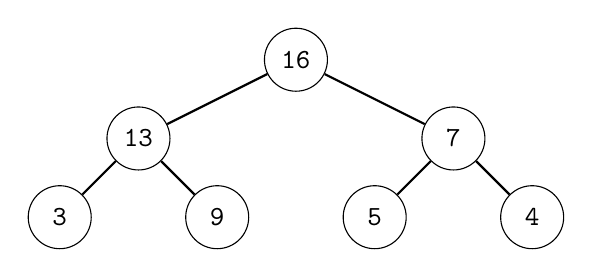
\begin{tikzpicture}
\node at (3,-1) [circle,draw,minimum size=8mm] (C) {\texttt{16}};
\node at (1,-2) [circle,draw,minimum size=8mm] (F) {\texttt{13}};
\node at (5,-2) [circle,draw,minimum size=8mm] (G) {\texttt{7}};
\node at (0,-3) [circle,draw,minimum size=8mm] (L) {\texttt{3}};
\node at (2,-3) [circle,draw,minimum size=8mm] (M) {\texttt{9}};
\node at (4,-3) [circle,draw,minimum size=8mm] (N) {\texttt{5}};
\node at (6,-3) [circle,draw,minimum size=8mm] (O) {\texttt{4}};
\draw [-,thick] (C) -- (G);
\draw [-,thick] (C) -- (F);
\draw [-,thick] (F) -- (L);
\draw [-,thick] (F) -- (M);
\draw [-,thick] (G) -- (N);
\draw [-,thick] (G) -- (O);

;
\end{tikzpicture}
    
\end{center}



Going from 15 back to the root, the first node that is not balanced is 10.
At 10, going down, I have to take a right (at 10) and then left (at 18).
This is the right-left case.
So I have to do a right rotation (at 18) and then a left rotation (at 10).
On doing a right rotation at 18, I get

\begin{center}
\begin{tikzpicture}

\fill[white] (0.0, 0.0) circle (0.3);
\node [line width=0.03cm,black,minimum size=0.57cm,draw,circle] at (0.0,0.0)(5){};\draw (0.0, 0.0) node[color=black] {\texttt{5}};
\fill[white] (-3.0, -1.0) circle (0.3);
\node [line width=0.03cm,black,minimum size=0.57cm,draw,circle] at (-3.0,-1.0)(2){};\draw (-3.0, -1.0) node[color=black] {\texttt{2}};
\fill[white] (3.0, -1.0) circle (0.3);
\node [line width=0.03cm,black,minimum size=0.57cm,draw,circle] at (3.0,-1.0)(10){};\draw (3.0, -1.0) node[color=black] {\texttt{10}};
\fill[white] (-4.5, -2.0) circle (0.3);
\node [line width=0.03cm,black,minimum size=0.57cm,draw,circle] at (-4.5,-2.0)(0){};\draw (-4.5, -2.0) node[color=black] {\texttt{0}};
\fill[white] (-1.5, -2.0) circle (0.3);
\node [line width=0.03cm,black,minimum size=0.57cm,draw,circle] at (-1.5,-2.0)(3){};\draw (-1.5, -2.0) node[color=black] {\texttt{3}};
\fill[white] (4.5, -2.0) circle (0.3);
\node [line width=0.03cm,black,minimum size=0.57cm,draw,circle] at (4.5,-2.0)(15){};\draw (4.5, -2.0) node[color=black] {\texttt{15}};
\fill[white] (5.25, -3.0) circle (0.3);
\node [line width=0.03cm,black,minimum size=0.57cm,draw,circle] at (5.25,-3.0)(18){};\draw (5.25, -3.0) node[color=black] {\texttt{18}};\draw[line width=0.03cm,black,->,>=triangle 60] (5) to  (2);
\draw[line width=0.03cm,black,->,>=triangle 60] (5) to  (10);
\draw[line width=0.03cm,black,->,>=triangle 60] (10) to  (15);
\draw[line width=0.03cm,black,->,>=triangle 60] (2) to  (0);
\draw[line width=0.03cm,black,->,>=triangle 60] (2) to  (3);
\draw[line width=0.03cm,black,->,>=triangle 60] (15) to  (18);
\end{tikzpicture}

\end{center}



and after a left rotation at 10, voila, I get

\begin{center}
\begin{tikzpicture}

\fill[white] (0.0, 0.0) circle (0.3);
\node [line width=0.03cm,black,minimum size=0.57cm,draw,circle] at (0.0,0.0)(5){};\draw (0.0, 0.0) node[color=black] {\texttt{5}};
\fill[white] (-3.0, -1.0) circle (0.3);
\node [line width=0.03cm,black,minimum size=0.57cm,draw,circle] at (-3.0,-1.0)(2){};\draw (-3.0, -1.0) node[color=black] {\texttt{2}};
\fill[white] (3.0, -1.0) circle (0.3);
\node [line width=0.03cm,black,minimum size=0.57cm,draw,circle] at (3.0,-1.0)(15){};\draw (3.0, -1.0) node[color=black] {\texttt{15}};
\fill[white] (-4.5, -2.0) circle (0.3);
\node [line width=0.03cm,black,minimum size=0.57cm,draw,circle] at (-4.5,-2.0)(0){};\draw (-4.5, -2.0) node[color=black] {\texttt{0}};
\fill[white] (-1.5, -2.0) circle (0.3);
\node [line width=0.03cm,black,minimum size=0.57cm,draw,circle] at (-1.5,-2.0)(3){};\draw (-1.5, -2.0) node[color=black] {\texttt{3}};
\fill[white] (1.5, -2.0) circle (0.3);
\node [line width=0.03cm,black,minimum size=0.57cm,draw,circle] at (1.5,-2.0)(10){};\draw (1.5, -2.0) node[color=black] {\texttt{10}};
\fill[white] (4.5, -2.0) circle (0.3);
\node [line width=0.03cm,black,minimum size=0.57cm,draw,circle] at (4.5,-2.0)(18){};\draw (4.5, -2.0) node[color=black] {\texttt{18}};\draw[line width=0.03cm,black,->,>=triangle 60] (5) to  (2);
\draw[line width=0.03cm,black,->,>=triangle 60] (5) to  (15);
\draw[line width=0.03cm,black,->,>=triangle 60] (15) to  (10);
\draw[line width=0.03cm,black,->,>=triangle 60] (15) to  (18);
\draw[line width=0.03cm,black,->,>=triangle 60] (2) to  (0);
\draw[line width=0.03cm,black,->,>=triangle 60] (2) to  (3);
\end{tikzpicture}

\end{center}



Note for AVL insertion, once you have found an unbalanced node,
you just need to work on that location (doing left or right or left-right or
right-left rotation) once.
The resulting tree is balanced again.
This assumes that you start out with an AVL tree.

The runtime of an insert into AVL is
\[
T(n) = O(\lg n)
\]
Why?
We know that worst runtime of BST insert is based on the height of the
tree.
Since the tree is balanced, the height is $O(\lg n)$.
After the insertion, we have to walk up the tree, which takes $O(\lg n)$ steps
and then perform one or two rotations, which takes $O(1)$ time.
Therefore altogether, AVL insertion has a worst runtime of $O(\lg n + \lg n + 1) =
O(\lg n)$.


\newpage
\subsection{Balance factor}

You notice that we need to compute the left height and right height
(i.e., height of
left subtree and height of right subtree) of nodes and compare which is larger.
It's convenient to store height information of a node
in the node.
I'll leave it to you to figure out how to update the heights of nodes in an
AVL tree when a node is inserted into it.



\newpage
\begin{ex}
Draw some AVL trees and label heights on the right of the all nodes.
Next, some inserts and recompute the heights of all nodes.
Do you see how to update the heights in general?
\end{ex}



\newpage
But there's another analogous method ... 

Note that since we're always comparing which
of left or right height is greater, we can simply store
\[
\text{(height of right subtree) $-$ (height of left subtree)}
\]
(or \lq\lq left minus right'') in a node.
This is frequently called the \defterm{balance factor} of the tree.
So if the balance factor is $+1$, then the right subtree has a greater height,
if the balance factor is $-1$, then the left subtree has a greater height,
and if the balance factor is $0$, then the left and right subtrees have the
same height.


\newpage
\begin{ex}
  Draw an AVL tree and compute the balance factor for each node.
  Next, perform an insert and see how to balance factors change.
  Can you figure out how to update balance factors in general?
  (Draw more pictures if necessary.)
\end{ex}

[HINT:
Leaf nodes have balance factor of 0 (duh).
During an insert, a node acquires a new child.
Suppose this is the node (value 10) with balance factor $b$
and the new child is going to be a left child:

\begin{center}
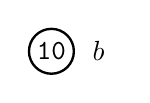
\begin{tikzpicture}

\fill[white] (0.0, 0.0) circle (0.3);
\node [line width=0.03cm,black,minimum size=0.57cm,draw,circle] at (0.0,0.0)(10){};\draw (0.0, 0.0) node[color=black] {\texttt{10}};
\fill[white] (0.6, 0.0) circle (0.3);
\node [draw=none,line width=0cm,black,minimum size=0.6cm,circle] at (0.6,0.0){};\draw (0.6, 0.0) node[color=black] {$b$};
\end{tikzpicture}

\end{center}



The number $b$ on the right of 10 is the balance factor.
The $b$ is either 0 or 1 (it can't be -1 since the new node
is going to be attached to 10 as a left child).
If $b$ is 0, then 10 does not have a
right child and if $b$ is 1, then 10 has a right child.
The balance factor of 10 decrements by 1:

\begin{center}
\begin{tikzpicture}


\node at (8,-1) [circle,draw,minimum size=8mm] (A) {\texttt{34}};
\node at (4,-2) [circle,draw,minimum size=8mm] (B) {\texttt{28}};
\node at (12,-2) [circle,draw,minimum size=8mm] (C) {\texttt{16}};
\node at (2,-3) [circle,draw,minimum size=8mm] (D) {\texttt{23}};
\node at (6,-3) [circle,draw,minimum size=8mm] (E) {\texttt{25}};
\node at (10,-3) [circle,draw,minimum size=8mm] (F) {\texttt{13}};
\node at (14,-3) [circle,draw,minimum size=8mm] (G) {\texttt{7}};
\node at (1,-4) [circle,draw,minimum size=8mm] (H) {\texttt{10}};
\node at (3,-4) [circle,draw,minimum size=8mm] (I) {\texttt{8}};
\node at (5,-4) [circle,draw,minimum size=8mm] (J) {\texttt{24}};
\node at (7,-4) [circle,draw,minimum size=8mm] (K) {\texttt{14}};
\node at (9,-4) [circle,draw,minimum size=8mm] (L) {\texttt{3}};
\node at (11,-4) [circle,draw,minimum size=8mm] (M) {\texttt{9}};
\node at (13,-4) [circle,draw,minimum size=8mm] (N) {\texttt{5}};
\node at (15,-4) [circle,draw,minimum size=8mm] (O) {\texttt{4}};
\node at (0,-5) [circle,draw,minimum size=8mm] (P) {\texttt{9}};
\draw [-,thick] (A) -- (B);
\draw [-,thick] (A) -- (C);
\draw [-,thick] (B) -- (D);
\draw [-,thick] (B) -- (E);
\draw [-,thick] (C) -- (G);
\draw [-,thick] (C) -- (F);
\draw [-,thick] (D) -- (H);
\draw [-,thick] (D) -- (I);
\draw [-,thick] (E) -- (J);
\draw [-,thick] (E) -- (K);
\draw [-,thick] (F) -- (L);
\draw [-,thick] (F) -- (M);
\draw [-,thick] (G) -- (N);
\draw [-,thick] (G) -- (O);
\draw [-,thick] (H) -- (P);

;

    \path[triangle 60-triangle 60,dashed] (K) edge [] (G);
\end{tikzpicture}

\end{center}



If the new node is attached to 10 as a right child, then we have
this update instead:

\begin{center}
\begin{tikzpicture}

\fill[white] (0.0, 0.0) circle (0.3);
\node [line width=0.03cm,black,minimum size=0.57cm,draw,circle] at (0.0,0.0)(10){};\draw (0.0, 0.0) node[color=black] {\texttt{10}};
\fill[white] (1.4, 0.0) circle (0.3);
\node [draw=none,line width=0cm,black,minimum size=0.6cm,circle] at (1.4,0.0){};\draw (1.4, 0.0) node[color=black] {$b \rightarrow b + 1$};
\fill[white] (0.75, -1.0) circle (0.3);
\node [line width=0.03cm,black,minimum size=0.57cm,draw,circle] at (0.75,-1.0)(5){};\draw (0.75, -1.0) node[color=black] {\texttt{5}};
\fill[white] (1.35, -1.0) circle (0.3);
\node [draw=none,line width=0cm,black,minimum size=0.6cm,circle] at (1.35,-1.0){};\draw (1.35, -1.0) node[color=black] {0};\draw[line width=0.03cm,black,->,>=triangle 60] (10) to  (5);
\end{tikzpicture}

\end{center}



Of course we update the balance factors on the path from the new node
to the root of the AVL tree.
So what do we do to the balance factor of the parent of 10?
Suppose 10 is a left child of 25
and their balance factors before the insert operation
are $b$ and  $b'$ respectively:


\begin{Verbatim}[frame=single, fontsize=\small]
#include <iostream>
#include <algorithm>
#include <vector>
#include <string>

void println(int v[], int size)
{
    std::string delim = "";
    std::cout << '{';
    for (int i = 0; i < size; ++i)
    {
        std::cout << delim << v[i];
        delim = ", ";
    }
    std::cout << "}\n";
}

int main()
{
    int x[] = {5,3,0,1,2,6,7,4};
    println(x, 8);
    std::make_heap(x, x + 8);
    println(x, 8);
    return 0;
}
\end{Verbatim}

\begin{console}[frame=single,fontsize=\small]
[student@localhost heap] g++ heapsort2.cpp -std=c++11
[student@localhost heap] ./a.out
{5, 3, 0, 1, 2, 6, 7, 4}
{7, 4, 6, 3, 2, 5, 0, 1}
\end{console}



The update on the balance factors of 10 and 25 is going to be:

\begin{center}
\begin{tikzpicture}

\fill[white] (0.0, 0.0) circle (0.3);
\node [line width=0.03cm,black,minimum size=0.57cm,draw,circle] at (0.0,0.0)(25){};\draw (0.0, 0.0) node[color=black] {\texttt{25}};
\fill[white] (1.5, 0.0) circle (0.3);
\node [draw=none,line width=0cm,black,minimum size=0.6cm,circle] at (1.5,0.0){};\draw (1.5, 0.0) node[color=black] {$b' \rightarrow b' - 1$};
\fill[white] (-1.5, -1.0) circle (0.3);
\node [line width=0.03cm,black,minimum size=0.57cm,draw,circle] at (-1.5,-1.0)(10){};\draw (-1.5, -1.0) node[color=black] {\texttt{10}};
\fill[white] (0.0, -1.0) circle (0.3);
\node [draw=none,line width=0cm,black,minimum size=0.6cm,circle] at (0.0,-1.0){};\draw (0.0, -1.0) node[color=black] {$b \rightarrow b - 1$};\draw[line width=0.03cm,black,->,>=triangle 60] (25) to  (10);
\end{tikzpicture}

\end{center}



In other words, if 10 is a left child and the balance factor of 10 decrements,
then the balance factor for the parent also decrements by 1.

All the above is saying is that if the height of the
left subtree at a node  grows by one, then the left subtree at its
parent also grows by one.
There's a similar update when the node is a right child:
If the node's balance factor increments by 1 and it's a right child,
then the parent's balance factor increments by 1.

Now what will happen if a new node is attached to node $n$ on the left,
but $n$ is a right child?

By drawing more pictures of AVL tree,
you should be able to figure out all the cases for the
balance factor updates. 
Of course once a balance factor hits $-2$ or $2$, you balance at that node
and update the balance factors of nodes affected.]


\newpage
\section{AVL delete}

AVL deletion is just BST deletion followed by rebalancing, just like AVL insertion.
The main difference is that, whereas for insert when one rebalancing act is enough
(left or right or left-right or right-left), for delete, you might need to rebalance
more than once.

Suppose I have this AVL tree:

\begin{center}
\begin{tikzpicture}


\node at (8,-1) [circle,draw,minimum size=8mm] (A) {\texttt{34}};
\node at (4,-2) [circle,draw,minimum size=8mm] (B) {\texttt{28}};
\node at (12,-2) [circle,draw,minimum size=8mm] (C) {\texttt{16}};
\node at (2,-3) [circle,draw,minimum size=8mm] (D) {\texttt{23}};
\node at (6,-3) [circle,draw,minimum size=8mm] (E) {\texttt{25}};
\node at (10,-3) [circle,draw,minimum size=8mm] (F) {\texttt{13}};
\node at (14,-3) [circle,draw,minimum size=8mm] (G) {\texttt{7}};
\node at (1,-4) [circle,draw,minimum size=8mm] (H) {\texttt{10}};
\node at (3,-4) [circle,draw,minimum size=8mm] (I) {\texttt{8}};
\node at (5,-4) [circle,draw,minimum size=8mm] (J) {\texttt{24}};
\node at (7,-4) [circle,draw,minimum size=8mm] (K) {\texttt{14}};
\node at (9,-4) [circle,draw,minimum size=8mm] (L) {\texttt{3}};
\node at (11,-4) [circle,draw,minimum size=8mm] (M) {\texttt{9}};
\node at (13,-4) [circle,draw,minimum size=8mm] (N) {\texttt{5}};
\node at (15,-4) [circle,draw,minimum size=8mm] (O) {\texttt{4}};
\node at (0,-5) [circle,draw,minimum size=8mm] (P) {\texttt{8}};
\node at (2,-5) [circle,draw,minimum size=8mm] (Q) {\texttt{9}};
\draw [-,thick] (A) -- (B);
\draw [-,thick] (A) -- (C);
\draw [-,thick] (B) -- (D);
\draw [-,thick] (B) -- (E);
\draw [-,thick] (C) -- (G);
\draw [-,thick] (C) -- (F);
\draw [-,thick] (D) -- (H);
\draw [-,thick] (D) -- (I);
\draw [-,thick] (E) -- (J);
\draw [-,thick] (E) -- (K);
\draw [-,thick] (F) -- (L);
\draw [-,thick] (F) -- (M);
\draw [-,thick] (G) -- (N);
\draw [-,thick] (G) -- (O);
\draw [-,thick] (H) -- (P);
\draw [-,thick] (H) -- (Q);

;

    \node (proot) at (8,0.5) {\texttt{proot}} ;\path [-triangle 60] (proot) edge[] (A);\node (p0) at (1,-5.5) {\texttt{p0}} ;\path [-triangle 60] (p0) edge[] (H);\node (p1) at (15,-5.5) {\texttt{p1}} ;\path [-triangle 60] (p1) edge[] (O);\node (p1) at (3,-5.5) {\texttt{p}} ;\path [-triangle 60] (p1) edge[] (I);
\end{tikzpicture}

\end{center}



(This is balanced.)
If I delete 12, I get this:

\begin{center}
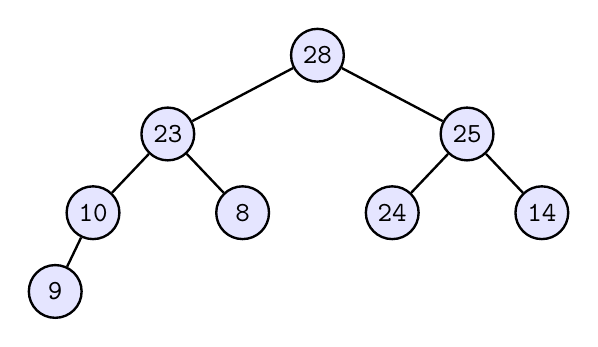
\begin{tikzpicture}

\fill[blue!10] (0.0, 0.0) circle (0.35);
\node [line width=0.03cm,black,minimum size=0.6699999999999999cm,draw,circle] at (0.0,0.0)(28){};\draw (0.0, 0.0) node[color=black] {\texttt{28}};
\fill[blue!10] (-1.9, -1.0) circle (0.35);
\node [line width=0.03cm,black,minimum size=0.6699999999999999cm,draw,circle] at (-1.9,-1.0)(23){};\draw (-1.9, -1.0) node[color=black] {\texttt{23}};
\fill[blue!10] (1.9, -1.0) circle (0.35);
\node [line width=0.03cm,black,minimum size=0.6699999999999999cm,draw,circle] at (1.9,-1.0)(25){};\draw (1.9, -1.0) node[color=black] {\texttt{25}};
\fill[blue!10] (-2.85, -2.0) circle (0.35);
\node [line width=0.03cm,black,minimum size=0.6699999999999999cm,draw,circle] at (-2.85,-2.0)(10){};\draw (-2.85, -2.0) node[color=black] {\texttt{10}};
\fill[blue!10] (-0.95, -2.0) circle (0.35);
\node [line width=0.03cm,black,minimum size=0.6699999999999999cm,draw,circle] at (-0.95,-2.0)(8){};\draw (-0.95, -2.0) node[color=black] {\texttt{8}};
\fill[blue!10] (0.95, -2.0) circle (0.35);
\node [line width=0.03cm,black,minimum size=0.6699999999999999cm,draw,circle] at (0.95,-2.0)(24){};\draw (0.95, -2.0) node[color=black] {\texttt{24}};
\fill[blue!10] (2.85, -2.0) circle (0.35);
\node [line width=0.03cm,black,minimum size=0.6699999999999999cm,draw,circle] at (2.85,-2.0)(14){};\draw (2.85, -2.0) node[color=black] {\texttt{14}};
\fill[blue!10] (-3.33, -3.0) circle (0.35);
\node [line width=0.03cm,black,minimum size=0.6699999999999999cm,draw,circle] at (-3.33,-3.0)(9){};\draw (-3.33, -3.0) node[color=black] {\texttt{9}};\draw[line width=0.03cm,black] (28) to  (23);
\draw[line width=0.03cm,black] (28) to  (25);
\draw[line width=0.03cm,black] (23) to  (10);
\draw[line width=0.03cm,black] (23) to  (8);
\draw[line width=0.03cm,black] (25) to  (24);
\draw[line width=0.03cm,black] (25) to  (14);
\draw[line width=0.03cm,black] (10) to  (9);
\end{tikzpicture}

\end{center}



which is again balanced -- I just need to check along the deletion path, from the root to the
parent of 10.

If I delete 15, I get this:

\begin{center}
\begin{tikzpicture}

\fill[white] (0.0, 0.0) circle (0.3);
\node [line width=0.03cm,black,minimum size=0.57cm,draw,circle] at (0.0,0.0)(10){};\draw (0.0, 0.0) node[color=black] {\texttt{10}};
\fill[white] (-3.0, -1.0) circle (0.3);
\node [line width=0.03cm,black,minimum size=0.57cm,draw,circle] at (-3.0,-1.0)(5){};\draw (-3.0, -1.0) node[color=black] {\texttt{5}};
\fill[white] (3.0, -1.0) circle (0.3);
\node [line width=0.03cm,black,minimum size=0.57cm,draw,circle] at (3.0,-1.0)(18){};\draw (3.0, -1.0) node[color=black] {\texttt{18}};
\fill[white] (-4.5, -2.0) circle (0.3);
\node [line width=0.03cm,black,minimum size=0.57cm,draw,circle] at (-4.5,-2.0)(0){};\draw (-4.5, -2.0) node[color=black] {\texttt{0}};
\fill[white] (-1.5, -2.0) circle (0.3);
\node [line width=0.03cm,black,minimum size=0.57cm,draw,circle] at (-1.5,-2.0)(7){};\draw (-1.5, -2.0) node[color=black] {\texttt{7}};
\fill[white] (-2.25, -3.0) circle (0.3);
\node [line width=0.03cm,black,minimum size=0.57cm,draw,circle] at (-2.25,-3.0)(6){};\draw (-2.25, -3.0) node[color=black] {\texttt{6}};
\fill[white] (-0.75, -3.0) circle (0.3);
\node [line width=0.03cm,black,minimum size=0.57cm,draw,circle] at (-0.75,-3.0)(8){};\draw (-0.75, -3.0) node[color=black] {\texttt{8}};\draw[line width=0.03cm,black,->,>=triangle 60] (10) to  (5);
\draw[line width=0.03cm,black,->,>=triangle 60] (10) to  (18);
\draw[line width=0.03cm,black,->,>=triangle 60] (5) to  (0);
\draw[line width=0.03cm,black,->,>=triangle 60] (5) to  (7);
\draw[line width=0.03cm,black,->,>=triangle 60] (7) to  (6);
\draw[line width=0.03cm,black,->,>=triangle 60] (7) to  (8);
\end{tikzpicture}

\end{center}



Going from 18 back to the root, I see that 10 is not balanced. 
Clearly the left subtree of 10 has a height that is too large.
Now, if I perform a right rotation at 10, I get

\begin{center}
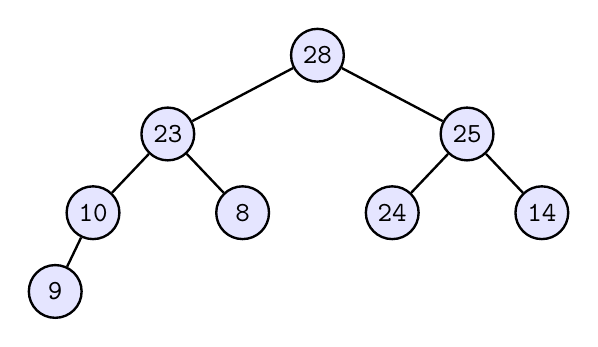
\begin{tikzpicture}

\fill[blue!10] (0.0, 0.0) circle (0.35);
\node [line width=0.03cm,black,minimum size=0.6699999999999999cm,draw,circle] at (0.0,0.0)(28){};\draw (0.0, 0.0) node[color=black] {\texttt{28}};
\fill[blue!10] (-1.9, -1.0) circle (0.35);
\node [line width=0.03cm,black,minimum size=0.6699999999999999cm,draw,circle] at (-1.9,-1.0)(23){};\draw (-1.9, -1.0) node[color=black] {\texttt{23}};
\fill[blue!10] (1.9, -1.0) circle (0.35);
\node [line width=0.03cm,black,minimum size=0.6699999999999999cm,draw,circle] at (1.9,-1.0)(25){};\draw (1.9, -1.0) node[color=black] {\texttt{25}};
\fill[blue!10] (-2.85, -2.0) circle (0.35);
\node [line width=0.03cm,black,minimum size=0.6699999999999999cm,draw,circle] at (-2.85,-2.0)(10){};\draw (-2.85, -2.0) node[color=black] {\texttt{10}};
\fill[blue!10] (-0.95, -2.0) circle (0.35);
\node [line width=0.03cm,black,minimum size=0.6699999999999999cm,draw,circle] at (-0.95,-2.0)(8){};\draw (-0.95, -2.0) node[color=black] {\texttt{8}};
\fill[blue!10] (0.95, -2.0) circle (0.35);
\node [line width=0.03cm,black,minimum size=0.6699999999999999cm,draw,circle] at (0.95,-2.0)(24){};\draw (0.95, -2.0) node[color=black] {\texttt{24}};
\fill[blue!10] (2.85, -2.0) circle (0.35);
\node [line width=0.03cm,black,minimum size=0.6699999999999999cm,draw,circle] at (2.85,-2.0)(14){};\draw (2.85, -2.0) node[color=black] {\texttt{14}};
\fill[blue!10] (-3.33, -3.0) circle (0.35);
\node [line width=0.03cm,black,minimum size=0.6699999999999999cm,draw,circle] at (-3.33,-3.0)(9){};\draw (-3.33, -3.0) node[color=black] {\texttt{9}};\draw[line width=0.03cm,black] (28) to  (23);
\draw[line width=0.03cm,black] (28) to  (25);
\draw[line width=0.03cm,black] (23) to  (10);
\draw[line width=0.03cm,black] (23) to  (8);
\draw[line width=0.03cm,black] (25) to  (24);
\draw[line width=0.03cm,black] (25) to  (14);
\draw[line width=0.03cm,black] (10) to  (9);
\end{tikzpicture}

\end{center}



This does not work!
The same location
(where 10 was and is now occupied by 5) is still unbalanced!!!
The reason is because the path $10\rightarrow 5\rightarrow 7\rightarrow 6$ (or $8$)
is the one that is causing the unbalancedness at 10:

\begin{center}
\begin{tikzpicture}

\fill[white] (0.0, 0.0) circle (0.3);
\node [line width=0.03cm,black,minimum size=0.57cm,draw,circle] at (0.0,0.0)(10){};\draw (0.0, 0.0) node[color=black] {\texttt{10}};
\fill[white] (-3.0, -1.0) circle (0.3);
\node [line width=0.03cm,black,minimum size=0.57cm,draw,circle] at (-3.0,-1.0)(5){};\draw (-3.0, -1.0) node[color=black] {\texttt{5}};
\fill[white] (3.0, -1.0) circle (0.3);
\node [line width=0.03cm,black,minimum size=0.57cm,draw,circle] at (3.0,-1.0)(18){};\draw (3.0, -1.0) node[color=black] {\texttt{18}};
\fill[white] (-4.5, -2.0) circle (0.3);
\node [line width=0.03cm,black,minimum size=0.57cm,draw,circle] at (-4.5,-2.0)(0){};\draw (-4.5, -2.0) node[color=black] {\texttt{0}};
\fill[white] (-1.5, -2.0) circle (0.3);
\node [line width=0.03cm,black,minimum size=0.57cm,draw,circle] at (-1.5,-2.0)(7){};\draw (-1.5, -2.0) node[color=black] {\texttt{7}};
\fill[white] (-2.25, -3.0) circle (0.3);
\node [line width=0.03cm,black,minimum size=0.57cm,draw,circle] at (-2.25,-3.0)(6){};\draw (-2.25, -3.0) node[color=black] {\texttt{6}};
\fill[white] (-0.75, -3.0) circle (0.3);
\node [line width=0.03cm,black,minimum size=0.57cm,draw,circle] at (-0.75,-3.0)(8){};\draw (-0.75, -3.0) node[color=black] {\texttt{8}};\draw[line width=0.1cm,red,->,>=triangle 60] (10) to  (5);
\draw[line width=0.03cm,black,->,>=triangle 60] (10) to  (18);
\draw[line width=0.03cm,black,->,>=triangle 60] (5) to  (0);
\draw[line width=0.1cm,red,->,>=triangle 60] (5) to  (7);
\draw[line width=0.03cm,black,->,>=triangle 60] (7) to  (6);
\draw[line width=0.03cm,black,->,>=triangle 60] (7) to  (8);
\end{tikzpicture}

\end{center}



Since $10\rightarrow 5 \rightarrow 7$ is a left-right, we use the same idea from AVL
insert
and perform a left rotation at 5 and then a right rotation at 10.
After a left rotation at 5, we get


\begin{center}

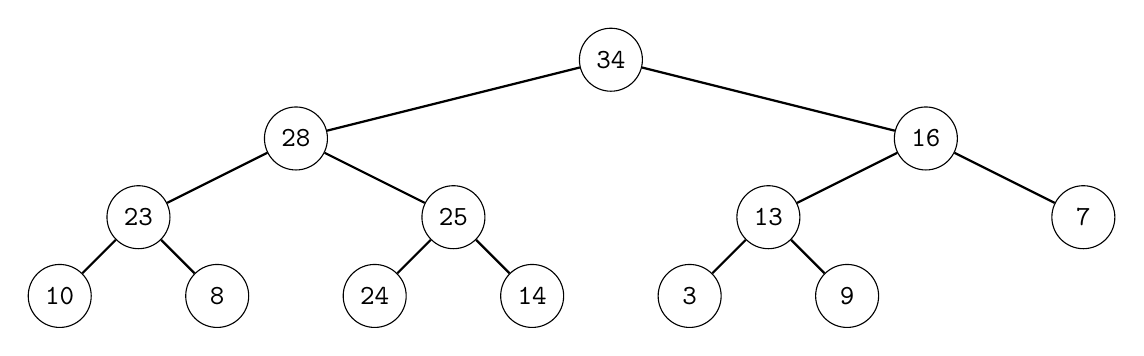
\begin{tikzpicture}
\node at (7,-1) [circle,draw,minimum size=8mm] (A) {\texttt{34}};
\node at (3,-2) [circle,draw,minimum size=8mm] (B) {\texttt{28}};
\node at (11,-2) [circle,draw,minimum size=8mm] (C) {\texttt{16}};
\node at (1,-3) [circle,draw,minimum size=8mm] (D) {\texttt{23}};
\node at (5,-3) [circle,draw,minimum size=8mm] (E) {\texttt{25}};
\node at (9,-3) [circle,draw,minimum size=8mm] (F) {\texttt{13}};
\node at (13,-3) [circle,draw,minimum size=8mm] (G) {\texttt{7}};
\node at (0,-4) [circle,draw,minimum size=8mm] (H) {\texttt{10}};
\node at (2,-4) [circle,draw,minimum size=8mm] (I) {\texttt{8}};
\node at (4,-4) [circle,draw,minimum size=8mm] (J) {\texttt{24}};
\node at (6,-4) [circle,draw,minimum size=8mm] (K) {\texttt{14}};
\node at (8,-4) [circle,draw,minimum size=8mm] (L) {\texttt{3}};
\node at (10,-4) [circle,draw,minimum size=8mm] (M) {\texttt{9}};
\draw [-,thick] (A) -- (B);
\draw [-,thick] (A) -- (C);
\draw [-,thick] (B) -- (D);
\draw [-,thick] (B) -- (E);
\draw [-,thick] (C) -- (G);
\draw [-,thick] (C) -- (F);
\draw [-,thick] (D) -- (H);
\draw [-,thick] (D) -- (I);
\draw [-,thick] (E) -- (J);
\draw [-,thick] (E) -- (K);
\draw [-,thick] (F) -- (L);
\draw [-,thick] (F) -- (M);

;
\end{tikzpicture}
    
\end{center}



And after a right rotation at 10, we get

\begin{center}
\begin{tikzpicture}


\node at (7,-1) [circle,draw,minimum size=8mm] (A) {\texttt{34}};
\node at (3,-2) [circle,draw,minimum size=8mm] (B) {\texttt{28}};
\node at (11,-2) [circle,draw,minimum size=8mm] (C) {\texttt{16}};
\node at (1,-3) [circle,draw,minimum size=8mm] (D) {\texttt{23}};
\node at (5,-3) [circle,draw,minimum size=8mm] (E) {\texttt{25}};
\node at (9,-3) [circle,draw,minimum size=8mm] (F) {\texttt{13}};
\node at (13,-3) [circle,draw,minimum size=8mm] (G) {\texttt{7}};
\node at (0,-4) [circle,draw,minimum size=8mm] (H) {\texttt{10}};
\node at (2,-4) [circle,draw,minimum size=8mm] (I) {\texttt{8}};
\node at (4,-4) [circle,draw,minimum size=8mm] (J) {\texttt{24}};
\node at (6,-4) [circle,draw,minimum size=8mm] (K) {\texttt{14}};
\node at (8,-4) [circle,draw,minimum size=8mm] (L) {\texttt{3}};
\node at (10,-4) [circle,draw,minimum size=8mm] (M) {\texttt{9}};
\node at (12,-4) [circle,draw,minimum size=8mm] (N) {\texttt{5}};
\draw [-,thick] (A) -- (B);
\draw [-,thick] (A) -- (C);
\draw [-,thick] (B) -- (D);
\draw [-,thick] (B) -- (E);
\draw [-,thick] (C) -- (G);
\draw [-,thick] (C) -- (F);
\draw [-,thick] (D) -- (H);
\draw [-,thick] (D) -- (I);
\draw [-,thick] (E) -- (J);
\draw [-,thick] (E) -- (K);
\draw [-,thick] (F) -- (L);
\draw [-,thick] (F) -- (M);
\draw [-,thick] (G) -- (N);

;

    \node (proot) at (7,0.5) {\texttt{proot}} ;\path [-triangle 60] (proot) edge[] (A);\node (p0) at (1,-4.5) {\texttt{p0}} ;\path [-triangle 60] (p0) edge[] (D);\node (p1) at (13,-4.5) {\texttt{p1}} ;\path [-triangle 60] (p1) edge[] (G);\node (p) at (13,-1.5) {\texttt{p}} ;\path [-triangle 60] (p) edge[] (G);
\end{tikzpicture}

\end{center}




Now node $7$, the previous location of $10$, balanced.
Since $7$ is now the root, we stop.
If $7$ is not the root, we have to keep going up and checking for
unbalanced nodes.
In general, you want to work your way up, starting with the
parent node of the node that was \textit{physically removed}.
This is \textit{not} necessarily the node you are deleting.
For instance recall that in some cases,
you need to delete the predecessor or successor of a node.
So in these cases, you start at the parent of the predecessor or successor
of the node and go up to the root.

Here's an example where after a delete, we need to rebalance at
two points.

Suppose you want to delete 8 from this tree,
using the move-predecessor-up:
\begin{center}
\begin{tikzpicture}

\fill[white] (0.0, 0.0) circle (0.3);
\node [line width=0.03cm,black,minimum size=0.57cm,draw,circle] at (0.0,0.0)(8){};\draw (0.0, 0.0) node[color=black] {\texttt{8}};
\fill[white] (-2.8, -1.0) circle (0.3);
\node [line width=0.03cm,black,minimum size=0.57cm,draw,circle] at (-2.8,-1.0)(5){};\draw (-2.8, -1.0) node[color=black] {\texttt{5}};
\fill[white] (2.8, -1.0) circle (0.3);
\node [line width=0.03cm,black,minimum size=0.57cm,draw,circle] at (2.8,-1.0)(15){};\draw (2.8, -1.0) node[color=black] {\texttt{15}};
\fill[white] (-4.2, -2.0) circle (0.3);
\node [line width=0.03cm,black,minimum size=0.57cm,draw,circle] at (-4.2,-2.0)(3){};\draw (-4.2, -2.0) node[color=black] {\texttt{3}};
\fill[white] (-1.4, -2.0) circle (0.3);
\node [line width=0.03cm,black,minimum size=0.57cm,draw,circle] at (-1.4,-2.0)(6){};\draw (-1.4, -2.0) node[color=black] {\texttt{6}};
\fill[white] (1.4, -2.0) circle (0.3);
\node [line width=0.03cm,black,minimum size=0.57cm,draw,circle] at (1.4,-2.0)(10){};\draw (1.4, -2.0) node[color=black] {\texttt{10}};
\fill[white] (4.2, -2.0) circle (0.3);
\node [line width=0.03cm,black,minimum size=0.57cm,draw,circle] at (4.2,-2.0)(22){};\draw (4.2, -2.0) node[color=black] {\texttt{22}};
\fill[white] (-3.5, -3.0) circle (0.3);
\node [line width=0.03cm,black,minimum size=0.57cm,draw,circle] at (-3.5,-3.0)(4){};\draw (-3.5, -3.0) node[color=black] {\texttt{4}};
\fill[white] (0.7, -3.0) circle (0.3);
\node [line width=0.03cm,black,minimum size=0.57cm,draw,circle] at (0.7,-3.0)(9){};\draw (0.7, -3.0) node[color=black] {\texttt{9}};
\fill[white] (2.1, -3.0) circle (0.3);
\node [line width=0.03cm,black,minimum size=0.57cm,draw,circle] at (2.1,-3.0)(12){};\draw (2.1, -3.0) node[color=black] {\texttt{12}};
\fill[white] (3.5, -3.0) circle (0.3);
\node [line width=0.03cm,black,minimum size=0.57cm,draw,circle] at (3.5,-3.0)(18){};\draw (3.5, -3.0) node[color=black] {\texttt{18}};
\fill[white] (4.9, -3.0) circle (0.3);
\node [line width=0.03cm,black,minimum size=0.57cm,draw,circle] at (4.9,-3.0)(28){};\draw (4.9, -3.0) node[color=black] {\texttt{28}};
\fill[white] (3.15, -4.0) circle (0.3);
\node [line width=0.03cm,black,minimum size=0.57cm,draw,circle] at (3.15,-4.0)(17){};\draw (3.15, -4.0) node[color=black] {\texttt{17}};
\fill[white] (3.8500000000000005, -4.0) circle (0.3);
\node [line width=0.03cm,black,minimum size=0.57cm,draw,circle] at (3.8500000000000005,-4.0)(19){};\draw (3.8500000000000005, -4.0) node[color=black] {\texttt{19}};\draw[line width=0.03cm,black,->,>=triangle 60] (8) to  (5);
\draw[line width=0.03cm,black,->,>=triangle 60] (8) to  (15);
\draw[line width=0.03cm,black,->,>=triangle 60] (5) to  (3);
\draw[line width=0.03cm,black,->,>=triangle 60] (5) to  (6);
\draw[line width=0.03cm,black,->,>=triangle 60] (15) to  (10);
\draw[line width=0.03cm,black,->,>=triangle 60] (15) to  (22);
\draw[line width=0.03cm,black,->,>=triangle 60] (3) to  (4);
\draw[line width=0.03cm,black,->,>=triangle 60] (10) to  (9);
\draw[line width=0.03cm,black,->,>=triangle 60] (10) to  (12);
\draw[line width=0.03cm,black,->,>=triangle 60] (22) to  (18);
\draw[line width=0.03cm,black,->,>=triangle 60] (22) to  (28);
\draw[line width=0.03cm,black,->,>=triangle 60] (18) to  (17);
\draw[line width=0.03cm,black,->,>=triangle 60] (18) to  (19);
\end{tikzpicture}

\end{center}


we get
\begin{center}
\begin{tikzpicture}

\fill[white] (0.0, 0.0) circle (0.3);
\node [line width=0.03cm,black,minimum size=0.57cm,draw,circle] at (0.0,0.0)(6){};\draw (0.0, 0.0) node[color=black] {\texttt{6}};
\fill[white] (-2.8, -1.0) circle (0.3);
\node [line width=0.03cm,black,minimum size=0.57cm,draw,circle] at (-2.8,-1.0)(5){};\draw (-2.8, -1.0) node[color=black] {\texttt{5}};
\fill[white] (2.8, -1.0) circle (0.3);
\node [line width=0.03cm,black,minimum size=0.57cm,draw,circle] at (2.8,-1.0)(15){};\draw (2.8, -1.0) node[color=black] {\texttt{15}};
\fill[white] (-4.2, -2.0) circle (0.3);
\node [line width=0.03cm,black,minimum size=0.57cm,draw,circle] at (-4.2,-2.0)(3){};\draw (-4.2, -2.0) node[color=black] {\texttt{3}};
\fill[white] (1.4, -2.0) circle (0.3);
\node [line width=0.03cm,black,minimum size=0.57cm,draw,circle] at (1.4,-2.0)(10){};\draw (1.4, -2.0) node[color=black] {\texttt{10}};
\fill[white] (4.2, -2.0) circle (0.3);
\node [line width=0.03cm,black,minimum size=0.57cm,draw,circle] at (4.2,-2.0)(22){};\draw (4.2, -2.0) node[color=black] {\texttt{22}};
\fill[white] (-3.5, -3.0) circle (0.3);
\node [line width=0.03cm,black,minimum size=0.57cm,draw,circle] at (-3.5,-3.0)(4){};\draw (-3.5, -3.0) node[color=black] {\texttt{4}};
\fill[white] (0.7, -3.0) circle (0.3);
\node [line width=0.03cm,black,minimum size=0.57cm,draw,circle] at (0.7,-3.0)(9){};\draw (0.7, -3.0) node[color=black] {\texttt{9}};
\fill[white] (2.1, -3.0) circle (0.3);
\node [line width=0.03cm,black,minimum size=0.57cm,draw,circle] at (2.1,-3.0)(12){};\draw (2.1, -3.0) node[color=black] {\texttt{12}};
\fill[white] (3.5, -3.0) circle (0.3);
\node [line width=0.03cm,black,minimum size=0.57cm,draw,circle] at (3.5,-3.0)(18){};\draw (3.5, -3.0) node[color=black] {\texttt{18}};
\fill[white] (4.9, -3.0) circle (0.3);
\node [line width=0.03cm,black,minimum size=0.57cm,draw,circle] at (4.9,-3.0)(28){};\draw (4.9, -3.0) node[color=black] {\texttt{28}};
\fill[white] (3.15, -4.0) circle (0.3);
\node [line width=0.03cm,black,minimum size=0.57cm,draw,circle] at (3.15,-4.0)(17){};\draw (3.15, -4.0) node[color=black] {\texttt{17}};
\fill[white] (3.8500000000000005, -4.0) circle (0.3);
\node [line width=0.03cm,black,minimum size=0.57cm,draw,circle] at (3.8500000000000005,-4.0)(19){};\draw (3.8500000000000005, -4.0) node[color=black] {\texttt{19}};\draw[line width=0.03cm,black,->,>=triangle 60] (6) to  (5);
\draw[line width=0.03cm,black,->,>=triangle 60] (6) to  (15);
\draw[line width=0.03cm,black,->,>=triangle 60] (5) to  (3);
\draw[line width=0.03cm,black,->,>=triangle 60] (15) to  (10);
\draw[line width=0.03cm,black,->,>=triangle 60] (15) to  (22);
\draw[line width=0.03cm,black,->,>=triangle 60] (3) to  (4);
\draw[line width=0.03cm,black,->,>=triangle 60] (10) to  (9);
\draw[line width=0.03cm,black,->,>=triangle 60] (10) to  (12);
\draw[line width=0.03cm,black,->,>=triangle 60] (22) to  (18);
\draw[line width=0.03cm,black,->,>=triangle 60] (22) to  (28);
\draw[line width=0.03cm,black,->,>=triangle 60] (18) to  (17);
\draw[line width=0.03cm,black,->,>=triangle 60] (18) to  (19);
\end{tikzpicture}

\end{center}


Now for the balancing.
We do \textit{not} start at the node with value 6 -- where 8 was.
Rather, \textit{we start at 5}, i.e., the parent of the predecessor of 8
that was removed (or moved)
in the case of move-predecessor-up
or the parent of the sucessor of 8
that was removed (or moved), depending on which one was moved.

We see that 5 is not balanced.
The left subtree of 5 has a larger height than the right.
Following two steps of the longest path in the left subtree
(in this case the only path), we see that the steps are left-right.
So we perform a left rotation at 3:
\begin{center}
\begin{tikzpicture}

\fill[white] (0.0, 0.0) circle (0.3);
\node [line width=0.03cm,black,minimum size=0.57cm,draw,circle] at (0.0,0.0)(6){};\draw (0.0, 0.0) node[color=black] {\texttt{6}};
\fill[white] (-2.8, -1.0) circle (0.3);
\node [line width=0.03cm,black,minimum size=0.57cm,draw,circle] at (-2.8,-1.0)(5){};\draw (-2.8, -1.0) node[color=black] {\texttt{5}};
\fill[white] (2.8, -1.0) circle (0.3);
\node [line width=0.03cm,black,minimum size=0.57cm,draw,circle] at (2.8,-1.0)(15){};\draw (2.8, -1.0) node[color=black] {\texttt{15}};
\fill[white] (-4.2, -2.0) circle (0.3);
\node [line width=0.03cm,black,minimum size=0.57cm,draw,circle] at (-4.2,-2.0)(4){};\draw (-4.2, -2.0) node[color=black] {\texttt{4}};
\fill[white] (1.4, -2.0) circle (0.3);
\node [line width=0.03cm,black,minimum size=0.57cm,draw,circle] at (1.4,-2.0)(10){};\draw (1.4, -2.0) node[color=black] {\texttt{10}};
\fill[white] (4.2, -2.0) circle (0.3);
\node [line width=0.03cm,black,minimum size=0.57cm,draw,circle] at (4.2,-2.0)(22){};\draw (4.2, -2.0) node[color=black] {\texttt{22}};
\fill[white] (-4.9, -3.0) circle (0.3);
\node [line width=0.03cm,black,minimum size=0.57cm,draw,circle] at (-4.9,-3.0)(3){};\draw (-4.9, -3.0) node[color=black] {\texttt{3}};
\fill[white] (0.7, -3.0) circle (0.3);
\node [line width=0.03cm,black,minimum size=0.57cm,draw,circle] at (0.7,-3.0)(9){};\draw (0.7, -3.0) node[color=black] {\texttt{9}};
\fill[white] (2.1, -3.0) circle (0.3);
\node [line width=0.03cm,black,minimum size=0.57cm,draw,circle] at (2.1,-3.0)(12){};\draw (2.1, -3.0) node[color=black] {\texttt{12}};
\fill[white] (3.5, -3.0) circle (0.3);
\node [line width=0.03cm,black,minimum size=0.57cm,draw,circle] at (3.5,-3.0)(18){};\draw (3.5, -3.0) node[color=black] {\texttt{18}};
\fill[white] (4.9, -3.0) circle (0.3);
\node [line width=0.03cm,black,minimum size=0.57cm,draw,circle] at (4.9,-3.0)(28){};\draw (4.9, -3.0) node[color=black] {\texttt{28}};
\fill[white] (3.15, -4.0) circle (0.3);
\node [line width=0.03cm,black,minimum size=0.57cm,draw,circle] at (3.15,-4.0)(17){};\draw (3.15, -4.0) node[color=black] {\texttt{17}};
\fill[white] (3.8500000000000005, -4.0) circle (0.3);
\node [line width=0.03cm,black,minimum size=0.57cm,draw,circle] at (3.8500000000000005,-4.0)(19){};\draw (3.8500000000000005, -4.0) node[color=black] {\texttt{19}};\draw[line width=0.03cm,black,->,>=triangle 60] (6) to  (5);
\draw[line width=0.03cm,black,->,>=triangle 60] (6) to  (15);
\draw[line width=0.03cm,black,->,>=triangle 60] (5) to  (4);
\draw[line width=0.03cm,black,->,>=triangle 60] (15) to  (10);
\draw[line width=0.03cm,black,->,>=triangle 60] (15) to  (22);
\draw[line width=0.03cm,black,->,>=triangle 60] (4) to  (3);
\draw[line width=0.03cm,black,->,>=triangle 60] (10) to  (9);
\draw[line width=0.03cm,black,->,>=triangle 60] (10) to  (12);
\draw[line width=0.03cm,black,->,>=triangle 60] (22) to  (18);
\draw[line width=0.03cm,black,->,>=triangle 60] (22) to  (28);
\draw[line width=0.03cm,black,->,>=triangle 60] (18) to  (17);
\draw[line width=0.03cm,black,->,>=triangle 60] (18) to  (19);
\end{tikzpicture}

\end{center}


and then a right rotation at 5 to get:
\begin{center}
\begin{tikzpicture}

\fill[white] (0.0, 0.0) circle (0.3);
\node [line width=0.03cm,black,minimum size=0.57cm,draw,circle] at (0.0,0.0)(6){};\draw (0.0, 0.0) node[color=black] {\texttt{6}};
\fill[white] (-2.8, -1.0) circle (0.3);
\node [line width=0.03cm,black,minimum size=0.57cm,draw,circle] at (-2.8,-1.0)(4){};\draw (-2.8, -1.0) node[color=black] {\texttt{4}};
\fill[white] (2.8, -1.0) circle (0.3);
\node [line width=0.03cm,black,minimum size=0.57cm,draw,circle] at (2.8,-1.0)(15){};\draw (2.8, -1.0) node[color=black] {\texttt{15}};
\fill[white] (-4.2, -2.0) circle (0.3);
\node [line width=0.03cm,black,minimum size=0.57cm,draw,circle] at (-4.2,-2.0)(3){};\draw (-4.2, -2.0) node[color=black] {\texttt{3}};
\fill[white] (-1.4, -2.0) circle (0.3);
\node [line width=0.03cm,black,minimum size=0.57cm,draw,circle] at (-1.4,-2.0)(5){};\draw (-1.4, -2.0) node[color=black] {\texttt{5}};
\fill[white] (1.4, -2.0) circle (0.3);
\node [line width=0.03cm,black,minimum size=0.57cm,draw,circle] at (1.4,-2.0)(10){};\draw (1.4, -2.0) node[color=black] {\texttt{10}};
\fill[white] (4.2, -2.0) circle (0.3);
\node [line width=0.03cm,black,minimum size=0.57cm,draw,circle] at (4.2,-2.0)(22){};\draw (4.2, -2.0) node[color=black] {\texttt{22}};
\fill[white] (0.7, -3.0) circle (0.3);
\node [line width=0.03cm,black,minimum size=0.57cm,draw,circle] at (0.7,-3.0)(9){};\draw (0.7, -3.0) node[color=black] {\texttt{9}};
\fill[white] (2.1, -3.0) circle (0.3);
\node [line width=0.03cm,black,minimum size=0.57cm,draw,circle] at (2.1,-3.0)(12){};\draw (2.1, -3.0) node[color=black] {\texttt{12}};
\fill[white] (3.5, -3.0) circle (0.3);
\node [line width=0.03cm,black,minimum size=0.57cm,draw,circle] at (3.5,-3.0)(18){};\draw (3.5, -3.0) node[color=black] {\texttt{18}};
\fill[white] (4.9, -3.0) circle (0.3);
\node [line width=0.03cm,black,minimum size=0.57cm,draw,circle] at (4.9,-3.0)(28){};\draw (4.9, -3.0) node[color=black] {\texttt{28}};
\fill[white] (3.15, -4.0) circle (0.3);
\node [line width=0.03cm,black,minimum size=0.57cm,draw,circle] at (3.15,-4.0)(17){};\draw (3.15, -4.0) node[color=black] {\texttt{17}};
\fill[white] (3.8500000000000005, -4.0) circle (0.3);
\node [line width=0.03cm,black,minimum size=0.57cm,draw,circle] at (3.8500000000000005,-4.0)(19){};\draw (3.8500000000000005, -4.0) node[color=black] {\texttt{19}};\draw[line width=0.03cm,black,->,>=triangle 60] (6) to  (4);
\draw[line width=0.03cm,black,->,>=triangle 60] (6) to  (15);
\draw[line width=0.03cm,black,->,>=triangle 60] (4) to  (3);
\draw[line width=0.03cm,black,->,>=triangle 60] (4) to  (5);
\draw[line width=0.03cm,black,->,>=triangle 60] (15) to  (10);
\draw[line width=0.03cm,black,->,>=triangle 60] (15) to  (22);
\draw[line width=0.03cm,black,->,>=triangle 60] (10) to  (9);
\draw[line width=0.03cm,black,->,>=triangle 60] (10) to  (12);
\draw[line width=0.03cm,black,->,>=triangle 60] (22) to  (18);
\draw[line width=0.03cm,black,->,>=triangle 60] (22) to  (28);
\draw[line width=0.03cm,black,->,>=triangle 60] (18) to  (17);
\draw[line width=0.03cm,black,->,>=triangle 60] (18) to  (19);
\end{tikzpicture}

\end{center}


The location we were balancing now has value 7 (it was previously 5).
Now we move up to 6.
6 is not balanced.
Following two steps of the longest path into the right, i.e.,
$6 \rightarrow 15 \rightarrow 22$, which is the right-right case,
we perform a left rotation at 6 to get:
\begin{center}
\begin{tikzpicture}

\fill[white] (0.0, 0.0) circle (0.3);
\node [line width=0.03cm,black,minimum size=0.57cm,draw,circle] at (0.0,0.0)(15){};\draw (0.0, 0.0) node[color=black] {\texttt{15}};
\fill[white] (-2.8, -1.0) circle (0.3);
\node [line width=0.03cm,black,minimum size=0.57cm,draw,circle] at (-2.8,-1.0)(6){};\draw (-2.8, -1.0) node[color=black] {\texttt{6}};
\fill[white] (2.8, -1.0) circle (0.3);
\node [line width=0.03cm,black,minimum size=0.57cm,draw,circle] at (2.8,-1.0)(22){};\draw (2.8, -1.0) node[color=black] {\texttt{22}};
\fill[white] (-4.2, -2.0) circle (0.3);
\node [line width=0.03cm,black,minimum size=0.57cm,draw,circle] at (-4.2,-2.0)(4){};\draw (-4.2, -2.0) node[color=black] {\texttt{4}};
\fill[white] (-1.4, -2.0) circle (0.3);
\node [line width=0.03cm,black,minimum size=0.57cm,draw,circle] at (-1.4,-2.0)(10){};\draw (-1.4, -2.0) node[color=black] {\texttt{10}};
\fill[white] (1.4, -2.0) circle (0.3);
\node [line width=0.03cm,black,minimum size=0.57cm,draw,circle] at (1.4,-2.0)(18){};\draw (1.4, -2.0) node[color=black] {\texttt{18}};
\fill[white] (4.2, -2.0) circle (0.3);
\node [line width=0.03cm,black,minimum size=0.57cm,draw,circle] at (4.2,-2.0)(28){};\draw (4.2, -2.0) node[color=black] {\texttt{28}};
\fill[white] (-4.9, -3.0) circle (0.3);
\node [line width=0.03cm,black,minimum size=0.57cm,draw,circle] at (-4.9,-3.0)(3){};\draw (-4.9, -3.0) node[color=black] {\texttt{3}};
\fill[white] (-3.5, -3.0) circle (0.3);
\node [line width=0.03cm,black,minimum size=0.57cm,draw,circle] at (-3.5,-3.0)(5){};\draw (-3.5, -3.0) node[color=black] {\texttt{5}};
\fill[white] (-2.1, -3.0) circle (0.3);
\node [line width=0.03cm,black,minimum size=0.57cm,draw,circle] at (-2.1,-3.0)(9){};\draw (-2.1, -3.0) node[color=black] {\texttt{9}};
\fill[white] (-0.7, -3.0) circle (0.3);
\node [line width=0.03cm,black,minimum size=0.57cm,draw,circle] at (-0.7,-3.0)(12){};\draw (-0.7, -3.0) node[color=black] {\texttt{12}};
\fill[white] (0.7, -3.0) circle (0.3);
\node [line width=0.03cm,black,minimum size=0.57cm,draw,circle] at (0.7,-3.0)(17){};\draw (0.7, -3.0) node[color=black] {\texttt{17}};
\fill[white] (2.1, -3.0) circle (0.3);
\node [line width=0.03cm,black,minimum size=0.57cm,draw,circle] at (2.1,-3.0)(19){};\draw (2.1, -3.0) node[color=black] {\texttt{19}};\draw[line width=0.03cm,black,->,>=triangle 60] (6) to  (4);
\draw[line width=0.03cm,black,->,>=triangle 60] (6) to  (10);
\draw[line width=0.03cm,black,->,>=triangle 60] (4) to  (3);
\draw[line width=0.03cm,black,->,>=triangle 60] (4) to  (5);
\draw[line width=0.03cm,black,->,>=triangle 60] (15) to  (6);
\draw[line width=0.03cm,black,->,>=triangle 60] (15) to  (22);
\draw[line width=0.03cm,black,->,>=triangle 60] (10) to  (9);
\draw[line width=0.03cm,black,->,>=triangle 60] (10) to  (12);
\draw[line width=0.03cm,black,->,>=triangle 60] (22) to  (18);
\draw[line width=0.03cm,black,->,>=triangle 60] (22) to  (28);
\draw[line width=0.03cm,black,->,>=triangle 60] (18) to  (17);
\draw[line width=0.03cm,black,->,>=triangle 60] (18) to  (19);
\end{tikzpicture}

\end{center}


If we followed right-left at 6 (which is incorrect because this
follows the shorter subtree!!! ),
then we would have performed
two rotations, first a right rotation at 15 to get:
\begin{center}
\begin{tikzpicture}

\fill[white] (2.0, 0.0) circle (0.3);
\node [line width=0.03cm,black,minimum size=0.57cm,draw,circle] at (2.0,0.0)(6){};\draw (2.0, 0.0) node[color=black] {\texttt{6}};
\fill[white] (-1.2, -1.0) circle (0.3);
\node [line width=0.03cm,black,minimum size=0.57cm,draw,circle] at (-1.2,-1.0)(4){};\draw (-1.2, -1.0) node[color=black] {\texttt{4}};
\fill[white] (5.2, -1.0) circle (0.3);
\node [line width=0.03cm,black,minimum size=0.57cm,draw,circle] at (5.2,-1.0)(10){};\draw (5.2, -1.0) node[color=black] {\texttt{10}};
\fill[white] (-2.3, -2.0) circle (0.3);
\node [line width=0.03cm,black,minimum size=0.57cm,draw,circle] at (-2.3,-2.0)(3){};\draw (-2.3, -2.0) node[color=black] {\texttt{3}};
\fill[white] (-0.10000000000000002, -2.0) circle (0.3);
\node [line width=0.03cm,black,minimum size=0.57cm,draw,circle] at (-0.10000000000000002,-2.0)(5){};\draw (-0.10000000000000002, -2.0) node[color=black] {\texttt{5}};
\fill[white] (2.6, -2.0) circle (0.3);
\node [line width=0.03cm,black,minimum size=0.57cm,draw,circle] at (2.6,-2.0)(9){};\draw (2.6, -2.0) node[color=black] {\texttt{9}};
\fill[white] (7.8, -2.0) circle (0.3);
\node [line width=0.03cm,black,minimum size=0.57cm,draw,circle] at (7.8,-2.0)(15){};\draw (7.8, -2.0) node[color=black] {\texttt{15}};
\fill[white] (6.5, -3.0) circle (0.3);
\node [line width=0.03cm,black,minimum size=0.57cm,draw,circle] at (6.5,-3.0)(12){};\draw (6.5, -3.0) node[color=black] {\texttt{12}};
\fill[white] (9.1, -3.0) circle (0.3);
\node [line width=0.03cm,black,minimum size=0.57cm,draw,circle] at (9.1,-3.0)(22){};\draw (9.1, -3.0) node[color=black] {\texttt{22}};
\fill[white] (8.45, -4.0) circle (0.3);
\node [line width=0.03cm,black,minimum size=0.57cm,draw,circle] at (8.45,-4.0)(18){};\draw (8.45, -4.0) node[color=black] {\texttt{18}};
\fill[white] (9.75, -4.0) circle (0.3);
\node [line width=0.03cm,black,minimum size=0.57cm,draw,circle] at (9.75,-4.0)(28){};\draw (9.75, -4.0) node[color=black] {\texttt{28}};
\fill[white] (8.12, -5.0) circle (0.3);
\node [line width=0.03cm,black,minimum size=0.57cm,draw,circle] at (8.12,-5.0)(17){};\draw (8.12, -5.0) node[color=black] {\texttt{17}};
\fill[white] (8.78, -5.0) circle (0.3);
\node [line width=0.03cm,black,minimum size=0.57cm,draw,circle] at (8.78,-5.0)(19){};\draw (8.78, -5.0) node[color=black] {\texttt{19}};\draw[line width=0.03cm,black,->,>=triangle 60] (6) to  (4);
\draw[line width=0.03cm,black,->,>=triangle 60] (6) to  (10);
\draw[line width=0.03cm,black,->,>=triangle 60] (4) to  (3);
\draw[line width=0.03cm,black,->,>=triangle 60] (4) to  (5);
\draw[line width=0.03cm,black,->,>=triangle 60] (15) to  (12);
\draw[line width=0.03cm,black,->,>=triangle 60] (15) to  (22);
\draw[line width=0.03cm,black,->,>=triangle 60] (10) to  (9);
\draw[line width=0.03cm,black,->,>=triangle 60] (10) to  (15);
\draw[line width=0.03cm,black,->,>=triangle 60] (22) to  (18);
\draw[line width=0.03cm,black,->,>=triangle 60] (22) to  (28);
\draw[line width=0.03cm,black,->,>=triangle 60] (18) to  (17);
\draw[line width=0.03cm,black,->,>=triangle 60] (18) to  (19);
\end{tikzpicture}

\end{center}


and then a left rotation at 6 to get:
\begin{center}
\begin{tikzpicture}

\fill[white] (0.0, 0.0) circle (0.3);
\node [line width=0.03cm,black,minimum size=0.57cm,draw,circle] at (0.0,0.0)(10){};\draw (0.0, 0.0) node[color=black] {\texttt{10}};
\fill[white] (-2.8, -1.0) circle (0.3);
\node [line width=0.03cm,black,minimum size=0.57cm,draw,circle] at (-2.8,-1.0)(6){};\draw (-2.8, -1.0) node[color=black] {\texttt{6}};
\fill[white] (2.8, -1.0) circle (0.3);
\node [line width=0.03cm,black,minimum size=0.57cm,draw,circle] at (2.8,-1.0)(15){};\draw (2.8, -1.0) node[color=black] {\texttt{15}};
\fill[white] (-4.2, -2.0) circle (0.3);
\node [line width=0.03cm,black,minimum size=0.57cm,draw,circle] at (-4.2,-2.0)(4){};\draw (-4.2, -2.0) node[color=black] {\texttt{4}};
\fill[white] (-1.4, -2.0) circle (0.3);
\node [line width=0.03cm,black,minimum size=0.57cm,draw,circle] at (-1.4,-2.0)(9){};\draw (-1.4, -2.0) node[color=black] {\texttt{9}};
\fill[white] (1.4, -2.0) circle (0.3);
\node [line width=0.03cm,black,minimum size=0.57cm,draw,circle] at (1.4,-2.0)(12){};\draw (1.4, -2.0) node[color=black] {\texttt{12}};
\fill[white] (4.2, -2.0) circle (0.3);
\node [line width=0.03cm,black,minimum size=0.57cm,draw,circle] at (4.2,-2.0)(22){};\draw (4.2, -2.0) node[color=black] {\texttt{22}};
\fill[white] (-4.9, -3.0) circle (0.3);
\node [line width=0.03cm,black,minimum size=0.57cm,draw,circle] at (-4.9,-3.0)(3){};\draw (-4.9, -3.0) node[color=black] {\texttt{3}};
\fill[white] (-3.5, -3.0) circle (0.3);
\node [line width=0.03cm,black,minimum size=0.57cm,draw,circle] at (-3.5,-3.0)(5){};\draw (-3.5, -3.0) node[color=black] {\texttt{5}};
\fill[white] (3.5, -3.0) circle (0.3);
\node [line width=0.03cm,black,minimum size=0.57cm,draw,circle] at (3.5,-3.0)(18){};\draw (3.5, -3.0) node[color=black] {\texttt{18}};
\fill[white] (4.9, -3.0) circle (0.3);
\node [line width=0.03cm,black,minimum size=0.57cm,draw,circle] at (4.9,-3.0)(28){};\draw (4.9, -3.0) node[color=black] {\texttt{28}};
\fill[white] (3.15, -4.0) circle (0.3);
\node [line width=0.03cm,black,minimum size=0.57cm,draw,circle] at (3.15,-4.0)(17){};\draw (3.15, -4.0) node[color=black] {\texttt{17}};
\fill[white] (3.8500000000000005, -4.0) circle (0.3);
\node [line width=0.03cm,black,minimum size=0.57cm,draw,circle] at (3.8500000000000005,-4.0)(19){};\draw (3.8500000000000005, -4.0) node[color=black] {\texttt{19}};\draw[line width=0.03cm,black,->,>=triangle 60] (6) to  (4);
\draw[line width=0.03cm,black,->,>=triangle 60] (6) to  (9);
\draw[line width=0.03cm,black,->,>=triangle 60] (4) to  (3);
\draw[line width=0.03cm,black,->,>=triangle 60] (4) to  (5);
\draw[line width=0.03cm,black,->,>=triangle 60] (15) to  (12);
\draw[line width=0.03cm,black,->,>=triangle 60] (15) to  (22);
\draw[line width=0.03cm,black,->,>=triangle 60] (10) to  (6);
\draw[line width=0.03cm,black,->,>=triangle 60] (10) to  (15);
\draw[line width=0.03cm,black,->,>=triangle 60] (22) to  (18);
\draw[line width=0.03cm,black,->,>=triangle 60] (22) to  (28);
\draw[line width=0.03cm,black,->,>=triangle 60] (18) to  (17);
\draw[line width=0.03cm,black,->,>=triangle 60] (18) to  (19);
\end{tikzpicture}

\end{center}


This results in an unbalanced node at 15.
So in general, you want to follow the node which is unbalanced (as much as possible)
to determine which of the left-left, left-right, right-left, right-right
case for balancing you want to execute.
In terms of balance factor, you want to choose +1 (right is taller -- go right)
or $-1$ (left is taller -- go left) whenever possible.

\begin{ex}
  Starting with an empty AVL tree, perform the following:
  \begin{tightlist}
    \li AVL-insert 6
    \li AVL-insert 5
    \li AVL-insert 4
    \li AVL-insert 3
    \li AVL-insert 2
    \li AVL-insert 1
    \li AVL-insert 7
    \li AVL-insert 8
    \li AVL-insert 9
    \li AVL-insert 10
    \li AVL-insert 11
    \li AVL-insert 12
    \li AVL-delete 4
    \li AVL-delete 3
    \li AVL-delete 2
    \li AVL-delete 1
    \li AVL-delete 5
    \li AVL-delete 7
    \li AVL-delete 6
    \li AVL-delete 8
    \li AVL-delete 11
    \li AVL-delete 12
    \li AVL-delete 9
    \li AVL-delete 10
  \end{tightlist}
\end{ex}


\begin{ex}
  Draw all BSTs with values 0, 1, 2, 3, 4.
  How many are AVLs?
\end{ex}



\begin{ex} [Merge]
  Given two BSTs, $T_1$ and $T_2$, construct a BST $T$ containing all the values in
  $T_1$ and $T_2$.
\end{ex}


\begin{ex}
  \begin{tightlist}
  \item Design an experiment to compare the performance of insert, delete, find
  on BSTs and AVLs.
  \item Do the same as above, but now include binary search trees which
  are like AVL but the delete operation does not rebalance.
  \item Do the same as above, but now include binary search trees which
  are like AVL but the delete operation will only rebalance at most once.
  \end{tightlist}
\end{ex}
  


\begin{ex}
  A $k$-AVL tree is basically an AVL where
   nodes are allowed to have the
  absolute value of their height balance factor
  $\leq k$ without balancing.
  Once the factor is $> k$, it is balanced.
  So a $1$--AVL is our regular AVL.
  Study this type of trees. Start with $2$--AVL trees.
  \qed \end{ex}


\begin{ex}
  Study the following BST.
  When a node is initially create, it have a counter of 10.
  Whenever a node is visited during a search, insert, delete,
  the counter drops by 1.
  Accessing a node durng balancing does not decrement the count.
  After an insert or delete, excluding new nodes during insert,
  if the starting node has a counter of 0,
  rebalancing occurs with balance factors updated and counters of
  nodes on the balancing path with counter set to 10.
  \qed
\end{ex}
